\documentclass[twoside]{book}

% Packages required by doxygen
\usepackage{fixltx2e}
\usepackage{calc}
\usepackage{doxygen}
\usepackage[export]{adjustbox} % also loads graphicx
\usepackage{graphicx}
\usepackage[utf8]{inputenc}
\usepackage{makeidx}
\usepackage{multicol}
\usepackage{multirow}
\PassOptionsToPackage{warn}{textcomp}
\usepackage{textcomp}
\usepackage[nointegrals]{wasysym}
\usepackage[table]{xcolor}

% Font selection
\usepackage[T1]{fontenc}
\usepackage[scaled=.90]{helvet}
\usepackage{courier}
\usepackage{amssymb}
\usepackage{sectsty}
\renewcommand{\familydefault}{\sfdefault}
\allsectionsfont{%
  \fontseries{bc}\selectfont%
  \color{darkgray}%
}
\renewcommand{\DoxyLabelFont}{%
  \fontseries{bc}\selectfont%
  \color{darkgray}%
}
\newcommand{\+}{\discretionary{\mbox{\scriptsize$\hookleftarrow$}}{}{}}

% Page & text layout
\usepackage{geometry}
\geometry{%
  a4paper,%
  top=2.5cm,%
  bottom=2.5cm,%
  left=2.5cm,%
  right=2.5cm%
}
\tolerance=750
\hfuzz=15pt
\hbadness=750
\setlength{\emergencystretch}{15pt}
\setlength{\parindent}{0cm}
\setlength{\parskip}{3ex plus 2ex minus 2ex}
\makeatletter
\renewcommand{\paragraph}{%
  \@startsection{paragraph}{4}{0ex}{-1.0ex}{1.0ex}{%
    \normalfont\normalsize\bfseries\SS@parafont%
  }%
}
\renewcommand{\subparagraph}{%
  \@startsection{subparagraph}{5}{0ex}{-1.0ex}{1.0ex}{%
    \normalfont\normalsize\bfseries\SS@subparafont%
  }%
}
\makeatother

% Headers & footers
\usepackage{fancyhdr}
\pagestyle{fancyplain}
\fancyhead[LE]{\fancyplain{}{\bfseries\thepage}}
\fancyhead[CE]{\fancyplain{}{}}
\fancyhead[RE]{\fancyplain{}{\bfseries\leftmark}}
\fancyhead[LO]{\fancyplain{}{\bfseries\rightmark}}
\fancyhead[CO]{\fancyplain{}{}}
\fancyhead[RO]{\fancyplain{}{\bfseries\thepage}}
\fancyfoot[LE]{\fancyplain{}{}}
\fancyfoot[CE]{\fancyplain{}{}}
\fancyfoot[RE]{\fancyplain{}{\bfseries\scriptsize Generated by Doxygen }}
\fancyfoot[LO]{\fancyplain{}{\bfseries\scriptsize Generated by Doxygen }}
\fancyfoot[CO]{\fancyplain{}{}}
\fancyfoot[RO]{\fancyplain{}{}}
\renewcommand{\footrulewidth}{0.4pt}
\renewcommand{\chaptermark}[1]{%
  \markboth{#1}{}%
}
\renewcommand{\sectionmark}[1]{%
  \markright{\thesection\ #1}%
}

% Indices & bibliography
\usepackage{natbib}
\usepackage[titles]{tocloft}
\setcounter{tocdepth}{3}
\setcounter{secnumdepth}{5}
\makeindex

% Hyperlinks (required, but should be loaded last)
\usepackage{ifpdf}
\ifpdf
  \usepackage[pdftex,pagebackref=true]{hyperref}
\else
  \usepackage[ps2pdf,pagebackref=true]{hyperref}
\fi
\hypersetup{%
  colorlinks=true,%
  linkcolor=blue,%
  citecolor=blue,%
  unicode%
}

% Custom commands
\newcommand{\clearemptydoublepage}{%
  \newpage{\pagestyle{empty}\cleardoublepage}%
}

\usepackage{caption}
\captionsetup{labelsep=space,justification=centering,font={bf},singlelinecheck=off,skip=4pt,position=top}

%===== C O N T E N T S =====

\begin{document}

% Titlepage & ToC
\hypersetup{pageanchor=false,
             bookmarksnumbered=true,
             pdfencoding=unicode
            }
\pagenumbering{roman}
\begin{titlepage}
\vspace*{7cm}
\begin{center}%
{\Large B\+I\+C\+O\+R\+D\+ER \\[1ex]\large v0.\+0.\+1 }\\
\vspace*{1cm}
{\large Generated by Doxygen 1.8.11}\\
\end{center}
\end{titlepage}
\clearemptydoublepage
\tableofcontents
\clearemptydoublepage
\pagenumbering{arabic}
\hypersetup{pageanchor=true}

%--- Begin generated contents ---
\chapter{B\+I\+C\+O\+R\+D\+ER}
\label{index}\hypertarget{index}{}Copyright (c) 2016 -\/ Gray Cat Labs -\/ \href{https://graycat.io}{\tt https\+://graycat.\+io}

I put this project together for the O\+SH Park Bring A Hack meetup at the 2016 Bay Area Maker Faire. It\textquotesingle{}s Tricorder inspired, but can\textquotesingle{}t quite sense everything, so the name \char`\"{}\+Bicorder\char`\"{} seemed fitting. It currently has a 3-\/axis magnetometer, a relative humidity / temperature sensor and an infrared range finder. It uses a 128x32 pixel monochrome L\+CD from Newhaven, which is divided into left and right sections, each displaying one of\+:


\begin{DoxyItemize}
\item live plot of temperature (in Celsius)
\item live plot of relative humidity
\item live plot of magnetic field (Z-\/axis) in u\+Tesla
\item a compass display (using the mag X and Y)
\item a distance readout in cm
\end{DoxyItemize}

\subsection*{License}

Released under the M\+IT license. \begin{DoxyVerb}Permission is hereby granted, free of charge, to any person obtaining a copy
of this software and associated documentation files (the "Software"), to deal
in the Software without restriction, including without limitation the rights
to use, copy, modify, merge, publish, distribute, sublicense, and/or sell
copies of the Software, and to permit persons to whom the Software is
furnished to do so, subject to the following conditions:

The above copyright notice and this permission notice shall be included in
all copies or substantial portions of the Software.

THE SOFTWARE IS PROVIDED "AS IS", WITHOUT WARRANTY OF ANY KIND, EXPRESS OR
IMPLIED, INCLUDING BUT NOT LIMITED TO THE WARRANTIES OF MERCHANTABILITY,
FITNESS FOR A PARTICULAR PURPOSE AND NONINFRINGEMENT. IN NO EVENT SHALL THE
AUTHORS OR COPYRIGHT HOLDERS BE LIABLE FOR ANY CLAIM, DAMAGES OR OTHER
LIABILITY, WHETHER IN AN ACTION OF CONTRACT, TORT OR OTHERWISE, ARISING FROM,
OUT OF OR IN CONNECTION WITH THE SOFTWARE OR THE USE OR OTHER DEALINGS IN
THE SOFTWARE. \end{DoxyVerb}
 
\chapter{Data Structure Index}
\section{Data Structures}
Here are the data structures with brief descriptions\+:\begin{DoxyCompactList}
\item\contentsline{section}{\hyperlink{structC12832A__config}{C12832\+A\+\_\+config} }{\pageref{structC12832A__config}}{}
\item\contentsline{section}{\hyperlink{structHMC5883L}{H\+M\+C5883L} }{\pageref{structHMC5883L}}{}
\item\contentsline{section}{\hyperlink{structHTU21D}{H\+T\+U21D} }{\pageref{structHTU21D}}{}
\item\contentsline{section}{\hyperlink{structuCorder__Compass}{u\+Corder\+\_\+\+Compass} }{\pageref{structuCorder__Compass}}{}
\item\contentsline{section}{\hyperlink{structuCorder__plot}{u\+Corder\+\_\+plot} }{\pageref{structuCorder__plot}}{}
\end{DoxyCompactList}

\chapter{File Index}
\section{File List}
Here is a list of all documented files with brief descriptions\+:\begin{DoxyCompactList}
\item\contentsline{section}{\hyperlink{bicorder-compass_8h}{bicorder-\/compass.\+h} \\*A library for generating a compass display on the Bicorder }{\pageref{bicorder-compass_8h}}{}
\item\contentsline{section}{\hyperlink{bicorder-plotter_8h}{bicorder-\/plotter.\+h} \\*A library for generating generic live plots on the Bicorder }{\pageref{bicorder-plotter_8h}}{}
\item\contentsline{section}{\hyperlink{bicorder_8h}{bicorder.\+h} \\*Config header for the Gray Cat Labs Bicorder }{\pageref{bicorder_8h}}{}
\item\contentsline{section}{\hyperlink{eGFX__Driver__C12832A__LPC824_8h}{e\+G\+F\+X\+\_\+\+Driver\+\_\+\+C12832\+A\+\_\+\+L\+P\+C824.\+h} \\*An e\+G\+FX driver for the Newhaven Display C12832A on the N\+XP L\+P\+C824 (and probably other L\+P\+C8\+XX) A\+RM Cortex-\/\+M0+ }{\pageref{eGFX__Driver__C12832A__LPC824_8h}}{}
\item\contentsline{section}{\hyperlink{gcl-fixedpoint_8h}{gcl-\/fixedpoint.\+h} \\*Basic 32-\/ and 64-\/bit signed fixed point math library }{\pageref{gcl-fixedpoint_8h}}{}
\item\contentsline{section}{\hyperlink{hmc5883l_8h}{hmc5883l.\+h} \\*A library for the \hyperlink{structHMC5883L}{H\+M\+C5883L} 3-\/axis I2C magnetometer }{\pageref{hmc5883l_8h}}{}
\item\contentsline{section}{\hyperlink{htu21d_8h}{htu21d.\+h} \\*A library for the \hyperlink{structHMC5883L}{H\+M\+C5883L} 3-\/axis I2C magnetometer }{\pageref{htu21d_8h}}{}
\item\contentsline{section}{\hyperlink{MoonLander-i2c_8h}{Moon\+Lander-\/i2c.\+h} \\*Basic polling I2C master driver for the N\+XP L\+P\+C824 (and probably other L\+P\+C8\+XX) A\+RM Cortex-\/\+M0+ }{\pageref{MoonLander-i2c_8h}}{}
\item\contentsline{section}{\hyperlink{MoonLander_8h}{Moon\+Lander.\+h} \\*Config for the Gray Cat Labs Moon\+Lander }{\pageref{MoonLander_8h}}{}
\end{DoxyCompactList}

\chapter{Data Structure Documentation}
\hypertarget{structC12832A__config}{}\section{C12832\+A\+\_\+config Struct Reference}
\label{structC12832A__config}\index{C12832\+A\+\_\+config@{C12832\+A\+\_\+config}}
\subsection*{Data Fields}
\begin{DoxyCompactItemize}
\item 
L\+P\+C\+\_\+\+S\+P\+I\+\_\+T $\ast$ {\bfseries lpc\+\_\+spi}\hypertarget{structC12832A__config_ac564ed12472e3c7f1d5d53f3ad650b0a}{}\label{structC12832A__config_ac564ed12472e3c7f1d5d53f3ad650b0a}

\item 
uint8\+\_\+t {\bfseries a0\+\_\+pin}\hypertarget{structC12832A__config_a37fea61d5b6d4f639cd3e9d2b757d0fa}{}\label{structC12832A__config_a37fea61d5b6d4f639cd3e9d2b757d0fa}

\item 
uint8\+\_\+t {\bfseries rst\+\_\+pin}\hypertarget{structC12832A__config_a00a7e26c38945362ba76d3cadf40763d}{}\label{structC12832A__config_a00a7e26c38945362ba76d3cadf40763d}

\item 
uint8\+\_\+t {\bfseries ssel\+\_\+num}\hypertarget{structC12832A__config_afbd3f1c01d74289465b28f40cb2c4cf4}{}\label{structC12832A__config_afbd3f1c01d74289465b28f40cb2c4cf4}

\end{DoxyCompactItemize}


\subsection{Detailed Description}


Definition at line 84 of file e\+G\+F\+X\+\_\+\+Driver\+\_\+\+C12832\+A\+\_\+\+L\+P\+C824.\+h.



The documentation for this struct was generated from the following file\+:\begin{DoxyCompactItemize}
\item 
\hyperlink{eGFX__Driver__C12832A__LPC824_8h}{e\+G\+F\+X\+\_\+\+Driver\+\_\+\+C12832\+A\+\_\+\+L\+P\+C824.\+h}\end{DoxyCompactItemize}

\hypertarget{structHMC5883L}{}\section{H\+M\+C5883L Struct Reference}
\label{structHMC5883L}\index{H\+M\+C5883L@{H\+M\+C5883L}}


{\ttfamily \#include $<$hmc5883l.\+h$>$}

\subsection*{Data Fields}
\begin{DoxyCompactItemize}
\item 
L\+P\+C\+\_\+\+I2\+C\+\_\+T $\ast$ {\bfseries i2c}\hypertarget{structHMC5883L_ab2edde7020ce0365265e7ba6f71a3e8b}{}\label{structHMC5883L_ab2edde7020ce0365265e7ba6f71a3e8b}

\item 
uint8\+\_\+t {\bfseries connected}\hypertarget{structHMC5883L_ad80cc8a1634a07add5886a5e0df835ce}{}\label{structHMC5883L_ad80cc8a1634a07add5886a5e0df835ce}

\item 
\hyperlink{hmc5883l_8h_a741d6341bd7d31bf60ea406397fd4ffe}{H\+M\+C5883\+L\+\_\+range} {\bfseries range}\hypertarget{structHMC5883L_ab914a355b6eb48243fce1936702f3d7c}{}\label{structHMC5883L_ab914a355b6eb48243fce1936702f3d7c}

\item 
int16\+\_\+t {\bfseries divider}\hypertarget{structHMC5883L_a946047cdc4bf51d366c1aa0204c799af}{}\label{structHMC5883L_a946047cdc4bf51d366c1aa0204c799af}

\end{DoxyCompactItemize}


\subsection{Detailed Description}
An \hyperlink{structHMC5883L}{H\+M\+C5883L} object to be passed the the \hyperlink{structHMC5883L}{H\+M\+C5883L} routines. 

Definition at line 79 of file hmc5883l.\+h.



The documentation for this struct was generated from the following file\+:\begin{DoxyCompactItemize}
\item 
\hyperlink{hmc5883l_8h}{hmc5883l.\+h}\end{DoxyCompactItemize}

\hypertarget{structHTU21D}{}\section{H\+T\+U21D Struct Reference}
\label{structHTU21D}\index{H\+T\+U21D@{H\+T\+U21D}}


{\ttfamily \#include $<$htu21d.\+h$>$}

\subsection*{Data Fields}
\begin{DoxyCompactItemize}
\item 
L\+P\+C\+\_\+\+I2\+C\+\_\+T $\ast$ {\bfseries i2c}\hypertarget{structHTU21D_ab8e165e384bebdc26d983df9eb211556}{}\label{structHTU21D_ab8e165e384bebdc26d983df9eb211556}

\item 
uint8\+\_\+t {\bfseries connected}\hypertarget{structHTU21D_a31081cc186d88df29eaa666cdcb50ee1}{}\label{structHTU21D_a31081cc186d88df29eaa666cdcb50ee1}

\end{DoxyCompactItemize}


\subsection{Detailed Description}
An \hyperlink{structHTU21D}{H\+T\+U21D} object to be passed the the \hyperlink{structHTU21D}{H\+T\+U21D} routines. 

Definition at line 46 of file htu21d.\+h.



The documentation for this struct was generated from the following file\+:\begin{DoxyCompactItemize}
\item 
\hyperlink{htu21d_8h}{htu21d.\+h}\end{DoxyCompactItemize}

\hypertarget{structuCorder__Compass}{}\section{u\+Corder\+\_\+\+Compass Struct Reference}
\label{structuCorder__Compass}\index{u\+Corder\+\_\+\+Compass@{u\+Corder\+\_\+\+Compass}}
\subsection*{Data Fields}
\begin{DoxyCompactItemize}
\item 
int\+\_\+fp {\bfseries mag\+\_\+x}\hypertarget{structuCorder__Compass_af41d1cdaeeb99641aa280adacf2074dd}{}\label{structuCorder__Compass_af41d1cdaeeb99641aa280adacf2074dd}

\item 
int\+\_\+fp {\bfseries mag\+\_\+y}\hypertarget{structuCorder__Compass_ac29f03e0c84d9e4ff922482f0db83e07}{}\label{structuCorder__Compass_ac29f03e0c84d9e4ff922482f0db83e07}

\end{DoxyCompactItemize}


\subsection{Detailed Description}


Definition at line 41 of file bicorder-\/compass.\+h.



The documentation for this struct was generated from the following file\+:\begin{DoxyCompactItemize}
\item 
\hyperlink{bicorder-compass_8h}{bicorder-\/compass.\+h}\end{DoxyCompactItemize}

\hypertarget{structuCorder__plot}{}\section{u\+Corder\+\_\+plot Struct Reference}
\label{structuCorder__plot}\index{u\+Corder\+\_\+plot@{u\+Corder\+\_\+plot}}
\subsection*{Data Fields}
\begin{DoxyCompactItemize}
\item 
int32\+\_\+t {\bfseries y\+\_\+min}\hypertarget{structuCorder__plot_aae1a5fa07c39489be789419a6af21a9f}{}\label{structuCorder__plot_aae1a5fa07c39489be789419a6af21a9f}

\item 
int32\+\_\+t {\bfseries y\+\_\+max}\hypertarget{structuCorder__plot_acec39cd0622e5cd98445036ca9f0ff10}{}\label{structuCorder__plot_acec39cd0622e5cd98445036ca9f0ff10}

\item 
int32\+\_\+t {\bfseries data} \mbox{[}P\+L\+O\+T\+\_\+\+W\+I\+D\+TH\mbox{]}\hypertarget{structuCorder__plot_afcf0c27eb85cb070a1e7f700a194bc9a}{}\label{structuCorder__plot_afcf0c27eb85cb070a1e7f700a194bc9a}

\item 
uint8\+\_\+t {\bfseries start\+\_\+index}\hypertarget{structuCorder__plot_aa0f03e14034689bc17504814be34e587}{}\label{structuCorder__plot_aa0f03e14034689bc17504814be34e587}

\item 
char {\bfseries label} \mbox{[}P\+L\+O\+T\+\_\+\+L\+A\+B\+E\+L\+\_\+\+M\+A\+X\+\_\+\+L\+EN+1\mbox{]}\hypertarget{structuCorder__plot_a13119b44a9a3329503ef42f1d2c1e561}{}\label{structuCorder__plot_a13119b44a9a3329503ef42f1d2c1e561}

\item 
uint8\+\_\+t {\bfseries special\+\_\+value\+\_\+en}\hypertarget{structuCorder__plot_a3fe52054c7c8b1e41969a03ba602f097}{}\label{structuCorder__plot_a3fe52054c7c8b1e41969a03ba602f097}

\item 
int32\+\_\+t {\bfseries special\+\_\+value}\hypertarget{structuCorder__plot_aa4b62079041f14ea8082d80ad38764cd}{}\label{structuCorder__plot_aa4b62079041f14ea8082d80ad38764cd}

\item 
char {\bfseries special\+\_\+value\+\_\+msg} \mbox{[}P\+L\+O\+T\+\_\+\+S\+P\+E\+C\+I\+A\+L\+\_\+\+V\+A\+L\+U\+E\+\_\+\+M\+S\+G\+\_\+\+M\+A\+X\+\_\+\+L\+EN+1\mbox{]}\hypertarget{structuCorder__plot_a79bdf22868124a1e2e7961984e79b8be}{}\label{structuCorder__plot_a79bdf22868124a1e2e7961984e79b8be}

\item 
uint8\+\_\+t {\bfseries is\+\_\+fixed\+\_\+point}\hypertarget{structuCorder__plot_a13227dff4fd804415295f3b01f453d8a}{}\label{structuCorder__plot_a13227dff4fd804415295f3b01f453d8a}

\end{DoxyCompactItemize}


\subsection{Detailed Description}


Definition at line 49 of file bicorder-\/plotter.\+h.



The documentation for this struct was generated from the following file\+:\begin{DoxyCompactItemize}
\item 
\hyperlink{bicorder-plotter_8h}{bicorder-\/plotter.\+h}\end{DoxyCompactItemize}

\chapter{File Documentation}
\hypertarget{bicorder-compass_8h}{}\section{bicorder-\/compass.h File Reference}
\label{bicorder-compass_8h}\index{bicorder-\/compass.\+h@{bicorder-\/compass.\+h}}


A library for generating a compass display on the Bicorder.  


{\ttfamily \#include \char`\"{}gcl-\/fixedpoint.\+h\char`\"{}}\\*
{\ttfamily \#include \char`\"{}e\+G\+F\+X\+\_\+\+Data\+Types.\+h\char`\"{}}\\*
Include dependency graph for bicorder-\/compass.h\+:
\nopagebreak
\begin{figure}[H]
\begin{center}
\leavevmode
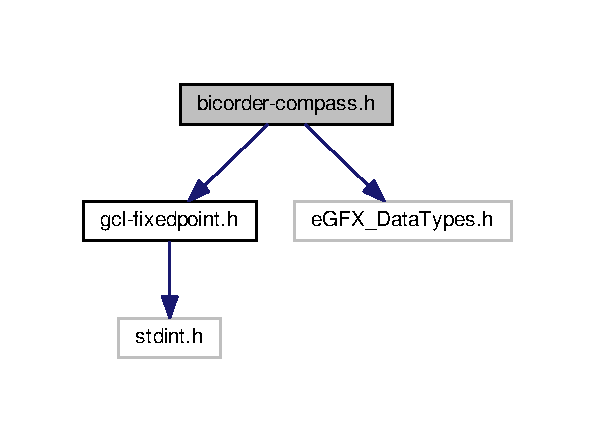
\includegraphics[width=286pt]{bicorder-compass_8h__incl}
\end{center}
\end{figure}
\subsection*{Data Structures}
\begin{DoxyCompactItemize}
\item 
struct \hyperlink{structuCorder__Compass}{u\+Corder\+\_\+\+Compass}
\end{DoxyCompactItemize}
\subsection*{Macros}
\begin{DoxyCompactItemize}
\item 
\#define {\bfseries C\+O\+M\+P\+A\+S\+S\+\_\+\+D\+E\+C\+L\+I\+N\+A\+T\+I\+ON}~(15)\hypertarget{bicorder-compass_8h_ae36b72028ffc628f320aba81b702036d}{}\label{bicorder-compass_8h_ae36b72028ffc628f320aba81b702036d}

\end{DoxyCompactItemize}
\subsection*{Enumerations}
\begin{DoxyCompactItemize}
\item 
enum \hyperlink{bicorder-compass_8h_a642eb4472a57f1a847ee101e3b7af5ba}{Compass\+\_\+direction} \{ \\*
{\bfseries C\+O\+M\+P\+A\+S\+S\+\_\+N}, 
{\bfseries C\+O\+M\+P\+A\+S\+S\+\_\+\+N\+NE}, 
{\bfseries C\+O\+M\+P\+A\+S\+S\+\_\+\+NE}, 
{\bfseries C\+O\+M\+P\+A\+S\+S\+\_\+\+E\+NE}, 
\\*
{\bfseries C\+O\+M\+P\+A\+S\+S\+\_\+E}, 
{\bfseries C\+O\+M\+P\+A\+S\+S\+\_\+\+E\+SE}, 
{\bfseries C\+O\+M\+P\+A\+S\+S\+\_\+\+SE}, 
{\bfseries C\+O\+M\+P\+A\+S\+S\+\_\+\+S\+SE}, 
\\*
{\bfseries C\+O\+M\+P\+A\+S\+S\+\_\+S}, 
{\bfseries C\+O\+M\+P\+A\+S\+S\+\_\+\+S\+SW}, 
{\bfseries C\+O\+M\+P\+A\+S\+S\+\_\+\+SW}, 
{\bfseries C\+O\+M\+P\+A\+S\+S\+\_\+\+W\+SW}, 
\\*
{\bfseries C\+O\+M\+P\+A\+S\+S\+\_\+W}, 
{\bfseries C\+O\+M\+P\+A\+S\+S\+\_\+\+W\+NW}, 
{\bfseries C\+O\+M\+P\+A\+S\+S\+\_\+\+NW}, 
{\bfseries C\+O\+M\+P\+A\+S\+S\+\_\+\+N\+NW}
 \}
\item 
enum \hyperlink{bicorder-compass_8h_a7e36843c53aaafda9795876e659ffe7b}{Compass\+\_\+side} \{ \hyperlink{bicorder-compass_8h_a7e36843c53aaafda9795876e659ffe7ba15cd36c342feb4b23e9a69bda67bcca8}{C\+O\+M\+P\+A\+S\+S\+\_\+\+L\+E\+FT}, 
\hyperlink{bicorder-compass_8h_a7e36843c53aaafda9795876e659ffe7ba61001c6c8cf0fa674b3039da44c1b005}{C\+O\+M\+P\+A\+S\+S\+\_\+\+R\+I\+G\+HT}
 \}
\end{DoxyCompactItemize}
\subsection*{Functions}
\begin{DoxyCompactItemize}
\item 
void \hyperlink{bicorder-compass_8h_a25d1189ee5127c18accd79eb68019cde}{Compass\+\_\+\+Init} (\hyperlink{structuCorder__Compass}{u\+Corder\+\_\+\+Compass} $\ast$compass)
\begin{DoxyCompactList}\small\item\em Initializes the given compass object. \end{DoxyCompactList}\item 
void \hyperlink{bicorder-compass_8h_a3e79bc358c252d3044f23b7e0766b54f}{Compass\+\_\+\+Update\+XY} (\hyperlink{structuCorder__Compass}{u\+Corder\+\_\+\+Compass} $\ast$compass, int\+\_\+fp x, int\+\_\+fp y)
\begin{DoxyCompactList}\small\item\em Sets the current X and Y magnetic field strength of the given compass object. \end{DoxyCompactList}\item 
uint16\+\_\+t \hyperlink{bicorder-compass_8h_a0fd608a7bf9aea8112efb03a4bc9bc5f}{Compass\+\_\+\+Calculate\+Heading} (\hyperlink{structuCorder__Compass}{u\+Corder\+\_\+\+Compass} $\ast$compass)
\begin{DoxyCompactList}\small\item\em Calculates and returns the current compass heading in degrees. \end{DoxyCompactList}\item 
\hyperlink{bicorder-compass_8h_a642eb4472a57f1a847ee101e3b7af5ba}{Compass\+\_\+direction} \hyperlink{bicorder-compass_8h_a1051f457631ee90b4f082177cf19d469}{Compass\+\_\+\+Heading\+To\+Direction} (uint16\+\_\+t heading)
\begin{DoxyCompactList}\small\item\em Returns the current compass direction from the given heading,. \end{DoxyCompactList}\item 
void \hyperlink{bicorder-compass_8h_a0ae721c1c17301cdf28bd0668a4f90af}{Compass\+\_\+\+Draw} (e\+G\+F\+X\+\_\+\+Image\+Plane $\ast$image, \hyperlink{structuCorder__Compass}{u\+Corder\+\_\+\+Compass} $\ast$compass, \hyperlink{bicorder-compass_8h_a7e36843c53aaafda9795876e659ffe7b}{Compass\+\_\+side} side)
\begin{DoxyCompactList}\small\item\em Returns the current compass direction from the given heading,. \end{DoxyCompactList}\end{DoxyCompactItemize}


\subsection{Detailed Description}
A library for generating a compass display on the Bicorder. 

\begin{DoxyAuthor}{Author}
Alex Hiam -\/ \href{mailto:alex@graycat.io}{\tt alex@graycat.\+io} 
\end{DoxyAuthor}


\subsection{Enumeration Type Documentation}
\index{bicorder-\/compass.\+h@{bicorder-\/compass.\+h}!Compass\+\_\+direction@{Compass\+\_\+direction}}
\index{Compass\+\_\+direction@{Compass\+\_\+direction}!bicorder-\/compass.\+h@{bicorder-\/compass.\+h}}
\subsubsection[{\texorpdfstring{Compass\+\_\+direction}{Compass_direction}}]{\setlength{\rightskip}{0pt plus 5cm}enum {\bf Compass\+\_\+direction}}\hypertarget{bicorder-compass_8h_a642eb4472a57f1a847ee101e3b7af5ba}{}\label{bicorder-compass_8h_a642eb4472a57f1a847ee101e3b7af5ba}
Compass headings as returned by \hyperlink{bicorder-compass_8h_a1051f457631ee90b4f082177cf19d469}{Compass\+\_\+\+Heading\+To\+Direction} 

Definition at line 79 of file bicorder-\/compass.\+h.

\index{bicorder-\/compass.\+h@{bicorder-\/compass.\+h}!Compass\+\_\+side@{Compass\+\_\+side}}
\index{Compass\+\_\+side@{Compass\+\_\+side}!bicorder-\/compass.\+h@{bicorder-\/compass.\+h}}
\subsubsection[{\texorpdfstring{Compass\+\_\+side}{Compass_side}}]{\setlength{\rightskip}{0pt plus 5cm}enum {\bf Compass\+\_\+side}}\hypertarget{bicorder-compass_8h_a7e36843c53aaafda9795876e659ffe7b}{}\label{bicorder-compass_8h_a7e36843c53aaafda9795876e659ffe7b}
Passed to \hyperlink{bicorder-compass_8h_a0ae721c1c17301cdf28bd0668a4f90af}{Compass\+\_\+\+Draw} to set which side of screen compass is displayed on \begin{Desc}
\item[Enumerator]\par
\begin{description}
\index{C\+O\+M\+P\+A\+S\+S\+\_\+\+L\+E\+FT@{C\+O\+M\+P\+A\+S\+S\+\_\+\+L\+E\+FT}!bicorder-\/compass.\+h@{bicorder-\/compass.\+h}}\index{bicorder-\/compass.\+h@{bicorder-\/compass.\+h}!C\+O\+M\+P\+A\+S\+S\+\_\+\+L\+E\+FT@{C\+O\+M\+P\+A\+S\+S\+\_\+\+L\+E\+FT}}\item[{\em 
C\+O\+M\+P\+A\+S\+S\+\_\+\+L\+E\+FT\hypertarget{bicorder-compass_8h_a7e36843c53aaafda9795876e659ffe7ba15cd36c342feb4b23e9a69bda67bcca8}{}\label{bicorder-compass_8h_a7e36843c53aaafda9795876e659ffe7ba15cd36c342feb4b23e9a69bda67bcca8}
}]Display compass on left side of screen. \index{C\+O\+M\+P\+A\+S\+S\+\_\+\+R\+I\+G\+HT@{C\+O\+M\+P\+A\+S\+S\+\_\+\+R\+I\+G\+HT}!bicorder-\/compass.\+h@{bicorder-\/compass.\+h}}\index{bicorder-\/compass.\+h@{bicorder-\/compass.\+h}!C\+O\+M\+P\+A\+S\+S\+\_\+\+R\+I\+G\+HT@{C\+O\+M\+P\+A\+S\+S\+\_\+\+R\+I\+G\+HT}}\item[{\em 
C\+O\+M\+P\+A\+S\+S\+\_\+\+R\+I\+G\+HT\hypertarget{bicorder-compass_8h_a7e36843c53aaafda9795876e659ffe7ba61001c6c8cf0fa674b3039da44c1b005}{}\label{bicorder-compass_8h_a7e36843c53aaafda9795876e659ffe7ba61001c6c8cf0fa674b3039da44c1b005}
}]Display compass on right side of screen. \end{description}
\end{Desc}


Definition at line 110 of file bicorder-\/compass.\+h.



\subsection{Function Documentation}
\index{bicorder-\/compass.\+h@{bicorder-\/compass.\+h}!Compass\+\_\+\+Calculate\+Heading@{Compass\+\_\+\+Calculate\+Heading}}
\index{Compass\+\_\+\+Calculate\+Heading@{Compass\+\_\+\+Calculate\+Heading}!bicorder-\/compass.\+h@{bicorder-\/compass.\+h}}
\subsubsection[{\texorpdfstring{Compass\+\_\+\+Calculate\+Heading(u\+Corder\+\_\+\+Compass $\ast$compass)}{Compass_CalculateHeading(uCorder_Compass *compass)}}]{\setlength{\rightskip}{0pt plus 5cm}uint16\+\_\+t Compass\+\_\+\+Calculate\+Heading (
\begin{DoxyParamCaption}
\item[{{\bf u\+Corder\+\_\+\+Compass} $\ast$}]{compass}
\end{DoxyParamCaption}
)}\hypertarget{bicorder-compass_8h_a0fd608a7bf9aea8112efb03a4bc9bc5f}{}\label{bicorder-compass_8h_a0fd608a7bf9aea8112efb03a4bc9bc5f}


Calculates and returns the current compass heading in degrees. 


\begin{DoxyParams}{Parameters}
{\em compass} & An initialized \hyperlink{structuCorder__Compass}{u\+Corder\+\_\+\+Compass} object\\
\hline
\end{DoxyParams}
\begin{DoxyReturn}{Returns}
Returns the current heading in degrees 
\end{DoxyReturn}
\index{bicorder-\/compass.\+h@{bicorder-\/compass.\+h}!Compass\+\_\+\+Draw@{Compass\+\_\+\+Draw}}
\index{Compass\+\_\+\+Draw@{Compass\+\_\+\+Draw}!bicorder-\/compass.\+h@{bicorder-\/compass.\+h}}
\subsubsection[{\texorpdfstring{Compass\+\_\+\+Draw(e\+G\+F\+X\+\_\+\+Image\+Plane $\ast$image, u\+Corder\+\_\+\+Compass $\ast$compass, Compass\+\_\+side side)}{Compass_Draw(eGFX_ImagePlane *image, uCorder_Compass *compass, Compass_side side)}}]{\setlength{\rightskip}{0pt plus 5cm}void Compass\+\_\+\+Draw (
\begin{DoxyParamCaption}
\item[{e\+G\+F\+X\+\_\+\+Image\+Plane $\ast$}]{image, }
\item[{{\bf u\+Corder\+\_\+\+Compass} $\ast$}]{compass, }
\item[{{\bf Compass\+\_\+side}}]{side}
\end{DoxyParamCaption}
)}\hypertarget{bicorder-compass_8h_a0ae721c1c17301cdf28bd0668a4f90af}{}\label{bicorder-compass_8h_a0ae721c1c17301cdf28bd0668a4f90af}


Returns the current compass direction from the given heading,. 


\begin{DoxyParams}{Parameters}
{\em heading} & Heading in degrees\\
\hline
\end{DoxyParams}
\begin{DoxyReturn}{Returns}
Returns a compass direction. 
\end{DoxyReturn}
\index{bicorder-\/compass.\+h@{bicorder-\/compass.\+h}!Compass\+\_\+\+Heading\+To\+Direction@{Compass\+\_\+\+Heading\+To\+Direction}}
\index{Compass\+\_\+\+Heading\+To\+Direction@{Compass\+\_\+\+Heading\+To\+Direction}!bicorder-\/compass.\+h@{bicorder-\/compass.\+h}}
\subsubsection[{\texorpdfstring{Compass\+\_\+\+Heading\+To\+Direction(uint16\+\_\+t heading)}{Compass_HeadingToDirection(uint16_t heading)}}]{\setlength{\rightskip}{0pt plus 5cm}{\bf Compass\+\_\+direction} Compass\+\_\+\+Heading\+To\+Direction (
\begin{DoxyParamCaption}
\item[{uint16\+\_\+t}]{heading}
\end{DoxyParamCaption}
)}\hypertarget{bicorder-compass_8h_a1051f457631ee90b4f082177cf19d469}{}\label{bicorder-compass_8h_a1051f457631ee90b4f082177cf19d469}


Returns the current compass direction from the given heading,. 


\begin{DoxyParams}{Parameters}
{\em heading} & Heading in degrees\\
\hline
\end{DoxyParams}
\begin{DoxyReturn}{Returns}
Returns a compass direction. 
\end{DoxyReturn}
\index{bicorder-\/compass.\+h@{bicorder-\/compass.\+h}!Compass\+\_\+\+Init@{Compass\+\_\+\+Init}}
\index{Compass\+\_\+\+Init@{Compass\+\_\+\+Init}!bicorder-\/compass.\+h@{bicorder-\/compass.\+h}}
\subsubsection[{\texorpdfstring{Compass\+\_\+\+Init(u\+Corder\+\_\+\+Compass $\ast$compass)}{Compass_Init(uCorder_Compass *compass)}}]{\setlength{\rightskip}{0pt plus 5cm}void Compass\+\_\+\+Init (
\begin{DoxyParamCaption}
\item[{{\bf u\+Corder\+\_\+\+Compass} $\ast$}]{compass}
\end{DoxyParamCaption}
)}\hypertarget{bicorder-compass_8h_a25d1189ee5127c18accd79eb68019cde}{}\label{bicorder-compass_8h_a25d1189ee5127c18accd79eb68019cde}


Initializes the given compass object. 


\begin{DoxyParams}{Parameters}
{\em compass} & The \hyperlink{structuCorder__Compass}{u\+Corder\+\_\+\+Compass} object to initialize \\
\hline
\end{DoxyParams}
\index{bicorder-\/compass.\+h@{bicorder-\/compass.\+h}!Compass\+\_\+\+Update\+XY@{Compass\+\_\+\+Update\+XY}}
\index{Compass\+\_\+\+Update\+XY@{Compass\+\_\+\+Update\+XY}!bicorder-\/compass.\+h@{bicorder-\/compass.\+h}}
\subsubsection[{\texorpdfstring{Compass\+\_\+\+Update\+X\+Y(u\+Corder\+\_\+\+Compass $\ast$compass, int\+\_\+fp x, int\+\_\+fp y)}{Compass_UpdateXY(uCorder_Compass *compass, int_fp x, int_fp y)}}]{\setlength{\rightskip}{0pt plus 5cm}void Compass\+\_\+\+Update\+XY (
\begin{DoxyParamCaption}
\item[{{\bf u\+Corder\+\_\+\+Compass} $\ast$}]{compass, }
\item[{int\+\_\+fp}]{x, }
\item[{int\+\_\+fp}]{y}
\end{DoxyParamCaption}
)}\hypertarget{bicorder-compass_8h_a3e79bc358c252d3044f23b7e0766b54f}{}\label{bicorder-compass_8h_a3e79bc358c252d3044f23b7e0766b54f}


Sets the current X and Y magnetic field strength of the given compass object. 


\begin{DoxyParams}{Parameters}
{\em compass} & An initialized \hyperlink{structuCorder__Compass}{u\+Corder\+\_\+\+Compass} object \\
\hline
{\em x} & The current X axis field strength \\
\hline
{\em y} & The current Y axis field strength \\
\hline
\end{DoxyParams}

\hypertarget{bicorder-plotter_8h}{}\section{bicorder-\/plotter.h File Reference}
\label{bicorder-plotter_8h}\index{bicorder-\/plotter.\+h@{bicorder-\/plotter.\+h}}


A library for generating generic live plots on the Bicorder.  


{\ttfamily \#include \char`\"{}e\+G\+F\+X\+\_\+\+Data\+Types.\+h\char`\"{}}\\*
Include dependency graph for bicorder-\/plotter.h\+:
\nopagebreak
\begin{figure}[H]
\begin{center}
\leavevmode
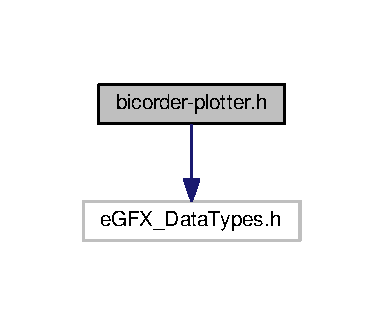
\includegraphics[width=184pt]{bicorder-plotter_8h__incl}
\end{center}
\end{figure}
\subsection*{Data Structures}
\begin{DoxyCompactItemize}
\item 
struct \hyperlink{structuCorder__plot}{u\+Corder\+\_\+plot}
\end{DoxyCompactItemize}
\subsection*{Macros}
\begin{DoxyCompactItemize}
\item 
\#define {\bfseries P\+L\+O\+T\+\_\+\+W\+I\+D\+TH}~40\hypertarget{bicorder-plotter_8h_a1fc4b17a5ce75463f2c6737654058dc9}{}\label{bicorder-plotter_8h_a1fc4b17a5ce75463f2c6737654058dc9}

\item 
\#define {\bfseries P\+L\+O\+T\+\_\+\+H\+E\+I\+G\+HT}~20\hypertarget{bicorder-plotter_8h_a2b49d5c686e9bd4f2ec6a3005eb798a5}{}\label{bicorder-plotter_8h_a2b49d5c686e9bd4f2ec6a3005eb798a5}

\item 
\#define {\bfseries P\+L\+O\+T\+\_\+\+M\+A\+R\+G\+I\+N\+\_\+\+L\+E\+FT}~20\hypertarget{bicorder-plotter_8h_a801b6f0ba4569299c3c6daf4e0defda5}{}\label{bicorder-plotter_8h_a801b6f0ba4569299c3c6daf4e0defda5}

\item 
\#define {\bfseries P\+L\+O\+T\+\_\+\+M\+A\+R\+G\+I\+N\+\_\+\+B\+O\+T\+T\+OM}~3\hypertarget{bicorder-plotter_8h_a2df60d2bc9bba913eb61dcf29214f6d3}{}\label{bicorder-plotter_8h_a2df60d2bc9bba913eb61dcf29214f6d3}

\item 
\#define {\bfseries P\+L\+O\+T\+\_\+\+G\+R\+A\+T\+I\+C\+L\+E\+\_\+\+W\+I\+D\+TH}~2\hypertarget{bicorder-plotter_8h_a58bdff8bea8d71f3d5b138d2b926ed76}{}\label{bicorder-plotter_8h_a58bdff8bea8d71f3d5b138d2b926ed76}

\item 
\#define {\bfseries P\+L\+O\+T\+\_\+\+N\+\_\+\+G\+R\+A\+T\+I\+C\+L\+E\+\_\+X}~5\hypertarget{bicorder-plotter_8h_afe7c4f9a4b7def188820c34befedd6c2}{}\label{bicorder-plotter_8h_afe7c4f9a4b7def188820c34befedd6c2}

\item 
\#define {\bfseries P\+L\+O\+T\+\_\+\+N\+\_\+\+G\+R\+A\+T\+I\+C\+L\+E\+\_\+Y}~5\hypertarget{bicorder-plotter_8h_ae49e5006579bd892974523899b206c1e}{}\label{bicorder-plotter_8h_ae49e5006579bd892974523899b206c1e}

\item 
\#define {\bfseries P\+L\+O\+T\+\_\+\+L\+A\+B\+E\+L\+\_\+\+M\+A\+X\+\_\+\+L\+EN}~10\hypertarget{bicorder-plotter_8h_aad7c802940ad17ae1b915ccef7f85d29}{}\label{bicorder-plotter_8h_aad7c802940ad17ae1b915ccef7f85d29}

\item 
\#define {\bfseries P\+L\+O\+T\+\_\+\+S\+P\+E\+C\+I\+A\+L\+\_\+\+V\+A\+L\+U\+E\+\_\+\+M\+S\+G\+\_\+\+M\+A\+X\+\_\+\+L\+EN}~5\hypertarget{bicorder-plotter_8h_a6b18117f2d9616dadc7b0d8cc04c4a0f}{}\label{bicorder-plotter_8h_a6b18117f2d9616dadc7b0d8cc04c4a0f}

\end{DoxyCompactItemize}
\subsection*{Enumerations}
\begin{DoxyCompactItemize}
\item 
enum {\bfseries Plot\+\_\+side} \{ {\bfseries P\+L\+O\+T\+\_\+\+L\+E\+FT}, 
{\bfseries P\+L\+O\+T\+\_\+\+R\+I\+G\+HT}
 \}\hypertarget{bicorder-plotter_8h_acce82b313701b0eca36d374e150f4a09}{}\label{bicorder-plotter_8h_acce82b313701b0eca36d374e150f4a09}

\end{DoxyCompactItemize}
\subsection*{Functions}
\begin{DoxyCompactItemize}
\item 
void {\bfseries Plot\+\_\+\+Init} (\hyperlink{structuCorder__plot}{u\+Corder\+\_\+plot} $\ast$plot, int32\+\_\+t y\+\_\+min, int32\+\_\+t y\+\_\+max, char $\ast$label, uint8\+\_\+t is\+\_\+fixed\+\_\+point)\hypertarget{bicorder-plotter_8h_a6fc1ecf8fe19709fbe8bdbb9b98b9f06}{}\label{bicorder-plotter_8h_a6fc1ecf8fe19709fbe8bdbb9b98b9f06}

\item 
void {\bfseries Plot\+\_\+\+Set\+Special\+Value} (\hyperlink{structuCorder__plot}{u\+Corder\+\_\+plot} $\ast$plot, int32\+\_\+t special\+\_\+value, char $\ast$msg)\hypertarget{bicorder-plotter_8h_a4ae0908e6a603750e088b87c3a098fe1}{}\label{bicorder-plotter_8h_a4ae0908e6a603750e088b87c3a098fe1}

\item 
void {\bfseries Plot\+\_\+\+Clear} (\hyperlink{structuCorder__plot}{u\+Corder\+\_\+plot} $\ast$plot)\hypertarget{bicorder-plotter_8h_a554a1bcc124c09b63ae03bbbbd210653}{}\label{bicorder-plotter_8h_a554a1bcc124c09b63ae03bbbbd210653}

\item 
void {\bfseries Plot\+\_\+\+Add\+Sample} (\hyperlink{structuCorder__plot}{u\+Corder\+\_\+plot} $\ast$plot, int32\+\_\+t sample)\hypertarget{bicorder-plotter_8h_ab5ce1c6e4771915429b750f013f69ea1}{}\label{bicorder-plotter_8h_ab5ce1c6e4771915429b750f013f69ea1}

\item 
void {\bfseries Plot\+\_\+\+Draw} (e\+G\+F\+X\+\_\+\+Image\+Plane $\ast$image, \hyperlink{structuCorder__plot}{u\+Corder\+\_\+plot} $\ast$plot, Plot\+\_\+side side)\hypertarget{bicorder-plotter_8h_aa77f4c18a3b6c579b14a4d6603fd971b}{}\label{bicorder-plotter_8h_aa77f4c18a3b6c579b14a4d6603fd971b}

\end{DoxyCompactItemize}


\subsection{Detailed Description}
A library for generating generic live plots on the Bicorder. 

\begin{DoxyAuthor}{Author}
Alex Hiam -\/ \href{mailto:alex@graycat.io}{\tt alex@graycat.\+io} 
\end{DoxyAuthor}

\hypertarget{bicorder_8h}{}\section{bicorder.\+h File Reference}
\label{bicorder_8h}\index{bicorder.\+h@{bicorder.\+h}}


Config header for the Gray Cat Labs Bicorder.  


{\ttfamily \#include \char`\"{}Moon\+Lander.\+h\char`\"{}}\\*
{\ttfamily \#include \char`\"{}chip.\+h\char`\"{}}\\*
Include dependency graph for bicorder.\+h\+:
\nopagebreak
\begin{figure}[H]
\begin{center}
\leavevmode
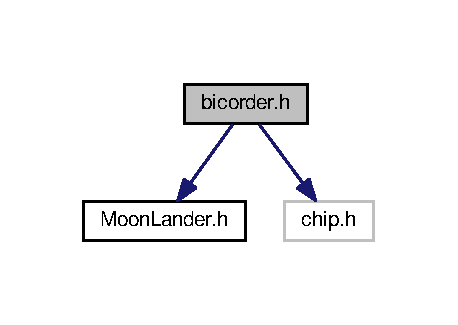
\includegraphics[width=220pt]{bicorder_8h__incl}
\end{center}
\end{figure}
\subsection*{Macros}
\begin{DoxyCompactItemize}
\item 
\#define {\bfseries B\+I\+C\+O\+R\+D\+E\+R\+\_\+\+H\+\_\+}\hypertarget{bicorder_8h_a08d46902b6156ecdb2e64f943c54e0c4}{}\label{bicorder_8h_a08d46902b6156ecdb2e64f943c54e0c4}

\item 
\#define {\bfseries S\+P\+I\+\_\+\+M\+O\+S\+I\+\_\+\+P\+IN}~Moon\+Lander\+\_\+\+I\+O1\hypertarget{bicorder_8h_a67d2c0b6e0ecbd0351958756e4830172}{}\label{bicorder_8h_a67d2c0b6e0ecbd0351958756e4830172}

\item 
\#define {\bfseries S\+P\+I\+\_\+\+S\+C\+K\+\_\+\+P\+IN}~Moon\+Lander\+\_\+\+I\+O2\hypertarget{bicorder_8h_aee89f642bb559e12db93e9f412ea185e}{}\label{bicorder_8h_aee89f642bb559e12db93e9f412ea185e}

\item 
\#define {\bfseries S\+P\+I\+\_\+\+P\+O\+RT}~L\+P\+C\+\_\+\+S\+P\+I0\hypertarget{bicorder_8h_a8112c985f7444e82198d7571ce0a9160}{}\label{bicorder_8h_a8112c985f7444e82198d7571ce0a9160}

\item 
\#define {\bfseries L\+C\+D\+\_\+\+A0\+\_\+\+P\+IN}~Moon\+Lander\+\_\+\+I\+O3\hypertarget{bicorder_8h_a2a7ab69e2d1e336875a8ba524a0059de}{}\label{bicorder_8h_a2a7ab69e2d1e336875a8ba524a0059de}

\item 
\#define {\bfseries L\+C\+D\+\_\+\+R\+S\+T\+\_\+\+P\+IN}~Moon\+Lander\+\_\+\+I\+O4\hypertarget{bicorder_8h_a9d11073f149e02e0a07937196d1e5a8e}{}\label{bicorder_8h_a9d11073f149e02e0a07937196d1e5a8e}

\item 
\#define {\bfseries L\+C\+D\+\_\+\+B\+A\+C\+K\+L\+I\+G\+HT}~Moon\+Lander\+\_\+\+I\+O7\hypertarget{bicorder_8h_ac059d24dfe9c1e1f7c07cb7869a1833b}{}\label{bicorder_8h_ac059d24dfe9c1e1f7c07cb7869a1833b}

\item 
\#define {\bfseries L\+C\+D\+\_\+\+C\+S\+\_\+\+P\+IN}~Moon\+Lander\+\_\+\+I\+O5\hypertarget{bicorder_8h_a50d72083b1ed4dd0bc2eaabb4a0332c8}{}\label{bicorder_8h_a50d72083b1ed4dd0bc2eaabb4a0332c8}

\item 
\#define {\bfseries L\+C\+D\+\_\+\+S\+S\+EL}~0\hypertarget{bicorder_8h_af9e3acc2829c7b09a6b0d6f675306fc5}{}\label{bicorder_8h_af9e3acc2829c7b09a6b0d6f675306fc5}

\item 
\#define {\bfseries S\+W\+M\+\_\+\+L\+C\+D\+\_\+\+CS}~S\+W\+M\+\_\+\+S\+P\+I0\+\_\+\+S\+S\+E\+L0\+\_\+\+IO\hypertarget{bicorder_8h_a49b26c4d61d70789efc83a3a4a0f9bbb}{}\label{bicorder_8h_a49b26c4d61d70789efc83a3a4a0f9bbb}

\item 
\#define {\bfseries S\+W\+\_\+\+L\+E\+FT}~Moon\+Lander\+\_\+\+I\+O9\hypertarget{bicorder_8h_aba3f4e7f3e0ffb7518057b10418829da}{}\label{bicorder_8h_aba3f4e7f3e0ffb7518057b10418829da}

\item 
\#define {\bfseries S\+W\+\_\+\+R\+I\+G\+HT}~Moon\+Lander\+\_\+\+I\+O10\hypertarget{bicorder_8h_a2cc8559702e048c339f68d72a94a5fa8}{}\label{bicorder_8h_a2cc8559702e048c339f68d72a94a5fa8}

\item 
\#define {\bfseries S\+W\+\_\+\+L\+E\+F\+T\+\_\+\+P\+I\+N\+I\+NT}~0\hypertarget{bicorder_8h_afce0ddec97e593a6d52f0b122545de38}{}\label{bicorder_8h_afce0ddec97e593a6d52f0b122545de38}

\item 
\#define {\bfseries S\+W\+\_\+\+L\+E\+F\+T\+\_\+\+P\+I\+N\+I\+N\+T\+CH}~(1$<$$<$S\+W\+\_\+\+L\+E\+F\+T\+\_\+\+P\+I\+N\+I\+NT)\hypertarget{bicorder_8h_a009a8f7991e0bcce27a2327f8142f90e}{}\label{bicorder_8h_a009a8f7991e0bcce27a2327f8142f90e}

\item 
\#define {\bfseries S\+W\+\_\+\+L\+E\+F\+T\+\_\+\+I\+R\+Qn}~P\+I\+N\+I\+N\+T0\+\_\+\+I\+R\+Qn\hypertarget{bicorder_8h_a229b1ffe9ebef6faec5184c2f26190fa}{}\label{bicorder_8h_a229b1ffe9ebef6faec5184c2f26190fa}

\item 
\#define {\bfseries S\+W\+\_\+\+L\+E\+F\+T\+\_\+\+I\+R\+Q\+Handler}~P\+I\+N\+\_\+\+I\+N\+T0\+\_\+\+I\+R\+Q\+Handler\hypertarget{bicorder_8h_a87ce5784299c30b9ecba809ad407f839}{}\label{bicorder_8h_a87ce5784299c30b9ecba809ad407f839}

\item 
\#define {\bfseries S\+W\+\_\+\+R\+I\+G\+H\+T\+\_\+\+P\+I\+N\+I\+NT}~1\hypertarget{bicorder_8h_a68adbdcf7db57b38492c36ccfcc1359a}{}\label{bicorder_8h_a68adbdcf7db57b38492c36ccfcc1359a}

\item 
\#define {\bfseries S\+W\+\_\+\+R\+I\+G\+H\+T\+\_\+\+P\+I\+N\+I\+N\+T\+CH}~(1$<$$<$S\+W\+\_\+\+R\+I\+G\+H\+T\+\_\+\+P\+I\+N\+I\+NT)\hypertarget{bicorder_8h_ac2f5041fc3fdfb946f851f2f80c8a4fa}{}\label{bicorder_8h_ac2f5041fc3fdfb946f851f2f80c8a4fa}

\item 
\#define {\bfseries S\+W\+\_\+\+R\+I\+G\+H\+T\+\_\+\+I\+R\+Qn}~P\+I\+N\+I\+N\+T1\+\_\+\+I\+R\+Qn\hypertarget{bicorder_8h_a6630a2cfdab264c352c5e7594f8a7661}{}\label{bicorder_8h_a6630a2cfdab264c352c5e7594f8a7661}

\item 
\#define {\bfseries S\+W\+\_\+\+R\+I\+G\+H\+T\+\_\+\+I\+R\+Q\+Handler}~P\+I\+N\+\_\+\+I\+N\+T1\+\_\+\+I\+R\+Q\+Handler\hypertarget{bicorder_8h_a00cf1e20dcab3eda9f913da73a38deef}{}\label{bicorder_8h_a00cf1e20dcab3eda9f913da73a38deef}

\item 
\#define {\bfseries S\+W\+\_\+\+D\+E\+B\+O\+U\+N\+C\+E\+\_\+\+MS}~300\hypertarget{bicorder_8h_acc6903857196bb786219de2f9418fd28}{}\label{bicorder_8h_acc6903857196bb786219de2f9418fd28}

\item 
\#define {\bfseries S\+W\+\_\+\+O\+F\+F\+\_\+\+H\+O\+L\+D\+\_\+\+T\+I\+M\+E\+\_\+\+MS}~2000\hypertarget{bicorder_8h_afb37b19bde7b58ddff34f54df5084c01}{}\label{bicorder_8h_afb37b19bde7b58ddff34f54df5084c01}

\item 
\#define {\bfseries R\+A\+N\+G\+E\+\_\+\+P\+O\+W\+E\+R\+\_\+\+P\+IN}~Moon\+Lander\+\_\+\+I\+O6\hypertarget{bicorder_8h_a556efe5ce50760ca8921c35222f03f76}{}\label{bicorder_8h_a556efe5ce50760ca8921c35222f03f76}

\item 
\#define {\bfseries R\+A\+N\+G\+E\+\_\+\+A\+IN}~Moon\+Lander\+\_\+\+I\+O8\+\_\+\+A\+DC\hypertarget{bicorder_8h_abca29e7df74f58d89979996f7185d79c}{}\label{bicorder_8h_abca29e7df74f58d89979996f7185d79c}

\item 
\#define {\bfseries A\+D\+C\+\_\+\+V\+\_\+\+P\+E\+R\+\_\+\+L\+SB}~0.\+0008056640625\hypertarget{bicorder_8h_a87def47694a4f309f4e9f573a422c774}{}\label{bicorder_8h_a87def47694a4f309f4e9f573a422c774}

\item 
\#define {\bfseries S\+E\+N\+S\+O\+R\+\_\+\+I2C}~L\+P\+C\+\_\+\+I2\+C0\hypertarget{bicorder_8h_af96e35c605829940b0c3e416bb054134}{}\label{bicorder_8h_af96e35c605829940b0c3e416bb054134}

\item 
\#define {\bfseries S\+A\+M\+P\+L\+E\+\_\+\+P\+E\+R\+I\+O\+D\+\_\+\+T\+E\+MP}~100\hypertarget{bicorder_8h_a863ad37eb86d65bd9419024a64d3de16}{}\label{bicorder_8h_a863ad37eb86d65bd9419024a64d3de16}

\item 
\#define {\bfseries S\+A\+M\+P\+L\+E\+\_\+\+P\+E\+R\+I\+O\+D\+\_\+\+RH}~100\hypertarget{bicorder_8h_a6b4ba9954598491b65150376b696a5d3}{}\label{bicorder_8h_a6b4ba9954598491b65150376b696a5d3}

\item 
\#define {\bfseries S\+A\+M\+P\+L\+E\+\_\+\+P\+E\+R\+I\+O\+D\+\_\+\+M\+AG}~100\hypertarget{bicorder_8h_a31eb182448e212b657bfe088492fd420}{}\label{bicorder_8h_a31eb182448e212b657bfe088492fd420}

\item 
\#define {\bfseries S\+A\+M\+P\+L\+E\+\_\+\+P\+E\+R\+I\+O\+D\+\_\+\+R\+A\+N\+GE}~250\hypertarget{bicorder_8h_a3e0a91d291473bbd46ee6173927dd84d}{}\label{bicorder_8h_a3e0a91d291473bbd46ee6173927dd84d}

\item 
\#define {\bfseries T\+I\+C\+K\+R\+A\+T\+E\+\_\+\+HZ}~1000\hypertarget{bicorder_8h_aa3a9dee7f854d803efded48120faadc8}{}\label{bicorder_8h_aa3a9dee7f854d803efded48120faadc8}

\item 
\#define {\bfseries M\+S\+\_\+\+P\+E\+R\+\_\+\+T\+I\+CK}~1\hypertarget{bicorder_8h_ae4e5a530999557f9d2687e40e8e8a7e1}{}\label{bicorder_8h_ae4e5a530999557f9d2687e40e8e8a7e1}

\item 
\#define {\bfseries B\+L\+I\+N\+K\+\_\+\+P\+E\+R\+I\+O\+D\+\_\+\+MS}~500\hypertarget{bicorder_8h_a8cfc4352ae90bdf0d97b6f3599f73acc}{}\label{bicorder_8h_a8cfc4352ae90bdf0d97b6f3599f73acc}

\item 
\#define {\bfseries I2\+C\+\_\+\+C\+L\+K\+\_\+\+D\+I\+V\+I\+D\+ER}~50\hypertarget{bicorder_8h_aeba29db21d6e7de94cf142c146ebac12}{}\label{bicorder_8h_aeba29db21d6e7de94cf142c146ebac12}

\item 
\#define {\bfseries I2\+C\+\_\+\+B\+I\+T\+R\+A\+TE}~\hyperlink{MoonLander-i2c_8h_a99b692076d07b714e6b130bdc715e3eea9a053bd0e23847d1237ee0dfbd0af724}{M\+O\+O\+N\+L\+A\+N\+D\+E\+R\+\_\+\+I2\+C\+\_\+100K}\hypertarget{bicorder_8h_afc53663507dcbb1496269cc8f33385c2}{}\label{bicorder_8h_afc53663507dcbb1496269cc8f33385c2}

\end{DoxyCompactItemize}
\subsection*{Enumerations}
\begin{DoxyCompactItemize}
\item 
enum {\bfseries u\+Corder\+\_\+display} \{ \\*
{\bfseries D\+I\+S\+P\+L\+A\+Y\+\_\+\+T\+E\+MP}, 
{\bfseries D\+I\+S\+P\+L\+A\+Y\+\_\+\+RH}, 
{\bfseries D\+I\+S\+P\+L\+A\+Y\+\_\+\+M\+AG}, 
{\bfseries D\+I\+S\+P\+L\+A\+Y\+\_\+\+C\+O\+M\+P\+A\+SS}, 
\\*
{\bfseries D\+I\+S\+P\+L\+A\+Y\+\_\+\+R\+A\+N\+GE}, 
{\bfseries N\+\_\+\+D\+I\+S\+P\+L\+A\+YS}
 \}\hypertarget{bicorder_8h_a59dcf494b7034c3099ba59cac7b5518f}{}\label{bicorder_8h_a59dcf494b7034c3099ba59cac7b5518f}

\end{DoxyCompactItemize}


\subsection{Detailed Description}
Config header for the Gray Cat Labs Bicorder. 

\begin{DoxyAuthor}{Author}
Alex Hiam -\/ \href{mailto:alex@graycat.io}{\tt alex@graycat.\+io} 
\end{DoxyAuthor}

\hypertarget{eGFX__Driver__C12832A__LPC824_8h}{}\section{e\+G\+F\+X\+\_\+\+Driver\+\_\+\+C12832\+A\+\_\+\+L\+P\+C824.\+h File Reference}
\label{eGFX__Driver__C12832A__LPC824_8h}\index{e\+G\+F\+X\+\_\+\+Driver\+\_\+\+C12832\+A\+\_\+\+L\+P\+C824.\+h@{e\+G\+F\+X\+\_\+\+Driver\+\_\+\+C12832\+A\+\_\+\+L\+P\+C824.\+h}}


An e\+G\+FX driver for the Newhaven Display C12832A on the N\+XP L\+P\+C824 (and probably other L\+P\+C8\+XX) A\+RM Cortex-\/\+M0+.  


{\ttfamily \#include \char`\"{}chip.\+h\char`\"{}}\\*
{\ttfamily \#include \char`\"{}e\+G\+F\+X\+\_\+\+Data\+Types.\+h\char`\"{}}\\*
Include dependency graph for e\+G\+F\+X\+\_\+\+Driver\+\_\+\+C12832\+A\+\_\+\+L\+P\+C824.\+h\+:
% FIG 0
This graph shows which files directly or indirectly include this file\+:
% FIG 1
\subsection*{Data Structures}
\begin{DoxyCompactItemize}
\item 
struct \hyperlink{structC12832A__config}{C12832\+A\+\_\+config}
\end{DoxyCompactItemize}
\subsection*{Macros}
\begin{DoxyCompactItemize}
\item 
\#define {\bfseries C12832\+A\+\_\+\+A0\+\_\+\+C\+MD}~0\hypertarget{eGFX__Driver__C12832A__LPC824_8h_a879778198d22df28beb69e97836c4d17}{}\label{eGFX__Driver__C12832A__LPC824_8h_a879778198d22df28beb69e97836c4d17}

\item 
\#define {\bfseries C12832\+A\+\_\+\+A0\+\_\+\+D\+A\+TA}~1\hypertarget{eGFX__Driver__C12832A__LPC824_8h_afcd32a60cefc6eefe852f6241ba73590}{}\label{eGFX__Driver__C12832A__LPC824_8h_afcd32a60cefc6eefe852f6241ba73590}

\item 
\#define {\bfseries C12832\+A\+\_\+\+S\+P\+I\+\_\+\+B\+I\+T\+R\+A\+TE}~5000000\hypertarget{eGFX__Driver__C12832A__LPC824_8h_a4063dd635a87638aced205ea8f87a693}{}\label{eGFX__Driver__C12832A__LPC824_8h_a4063dd635a87638aced205ea8f87a693}

\item 
\#define {\bfseries C12832\+A\+\_\+\+S\+P\+I\+\_\+\+C\+L\+O\+C\+K\+M\+O\+DE}~S\+P\+I\+\_\+\+C\+L\+O\+C\+K\+\_\+\+C\+P\+H\+A1\+\_\+\+C\+P\+O\+L1\hypertarget{eGFX__Driver__C12832A__LPC824_8h_a6a3fcbfebdb675f8bd1a85563a2edda1}{}\label{eGFX__Driver__C12832A__LPC824_8h_a6a3fcbfebdb675f8bd1a85563a2edda1}

\item 
\#define {\bfseries C12832\+A\+\_\+\+S\+P\+I\+\_\+\+D\+A\+T\+A\+B\+I\+TS}~8\hypertarget{eGFX__Driver__C12832A__LPC824_8h_af65729df488195cfb7cd648c037a49d7}{}\label{eGFX__Driver__C12832A__LPC824_8h_af65729df488195cfb7cd648c037a49d7}

\item 
\#define {\bfseries C12832\+A\+\_\+\+C\+M\+D\+\_\+\+D\+I\+S\+P\+L\+A\+Y\+\_\+\+ON}~0x\+AF\hypertarget{eGFX__Driver__C12832A__LPC824_8h_a351c3b06bac13da63162f0425f73e225}{}\label{eGFX__Driver__C12832A__LPC824_8h_a351c3b06bac13da63162f0425f73e225}

\item 
\#define {\bfseries C12832\+A\+\_\+\+C\+M\+D\+\_\+\+D\+I\+S\+P\+L\+A\+Y\+\_\+\+O\+FF}~0x\+AE\hypertarget{eGFX__Driver__C12832A__LPC824_8h_a81fcb92b112792f9fe6adcbe2165d6ca}{}\label{eGFX__Driver__C12832A__LPC824_8h_a81fcb92b112792f9fe6adcbe2165d6ca}

\item 
\#define {\bfseries C\+M\+D\+\_\+\+S\+E\+T\+\_\+\+D\+I\+S\+P\+\_\+\+S\+T\+A\+R\+T\+\_\+\+L\+I\+NE}~0x40\hypertarget{eGFX__Driver__C12832A__LPC824_8h_a0aadc0773d2c68985728aaeaf5242710}{}\label{eGFX__Driver__C12832A__LPC824_8h_a0aadc0773d2c68985728aaeaf5242710}

\item 
\#define {\bfseries C12832\+A\+\_\+\+C\+M\+D\+\_\+\+P\+A\+GE}~0x\+B0\hypertarget{eGFX__Driver__C12832A__LPC824_8h_a6a445734feff727499d564b04335d5cb}{}\label{eGFX__Driver__C12832A__LPC824_8h_a6a445734feff727499d564b04335d5cb}

\item 
\#define {\bfseries C12832\+A\+\_\+\+C\+M\+D\+\_\+\+C\+O\+L\+\_\+\+H\+I\+GH}~0x10\hypertarget{eGFX__Driver__C12832A__LPC824_8h_a5ccce757c209da252b2d991c6c1af881}{}\label{eGFX__Driver__C12832A__LPC824_8h_a5ccce757c209da252b2d991c6c1af881}

\item 
\#define {\bfseries C12832\+A\+\_\+\+C\+M\+D\+\_\+\+C\+O\+L\+\_\+\+L\+OW}~0x00\hypertarget{eGFX__Driver__C12832A__LPC824_8h_a874cebc621f397120486af542d6514b0}{}\label{eGFX__Driver__C12832A__LPC824_8h_a874cebc621f397120486af542d6514b0}

\item 
\#define {\bfseries C12832\+A\+\_\+\+C\+M\+D\+\_\+\+A\+D\+C\+\_\+\+N\+O\+R\+M\+AL}~0x\+A0\hypertarget{eGFX__Driver__C12832A__LPC824_8h_a9cf87e5d966a565e042f7f16b8a33932}{}\label{eGFX__Driver__C12832A__LPC824_8h_a9cf87e5d966a565e042f7f16b8a33932}

\item 
\#define {\bfseries C12832\+A\+\_\+\+C\+M\+D\+\_\+\+A\+D\+C\+\_\+\+R\+E\+V\+E\+R\+SE}~0x\+A1\hypertarget{eGFX__Driver__C12832A__LPC824_8h_ac81e88e310da329a3f53341a8084ff0a}{}\label{eGFX__Driver__C12832A__LPC824_8h_ac81e88e310da329a3f53341a8084ff0a}

\item 
\#define {\bfseries C12832\+A\+\_\+\+C\+M\+D\+\_\+\+D\+I\+S\+P\+\_\+\+N\+O\+R\+M\+AL}~0x\+A6\hypertarget{eGFX__Driver__C12832A__LPC824_8h_a077d9c374ff0a5ade2c5a41b3f13d873}{}\label{eGFX__Driver__C12832A__LPC824_8h_a077d9c374ff0a5ade2c5a41b3f13d873}

\item 
\#define {\bfseries C12832\+A\+\_\+\+C\+M\+D\+\_\+\+D\+I\+S\+P\+\_\+\+R\+E\+V\+E\+R\+SE}~0x\+A7\hypertarget{eGFX__Driver__C12832A__LPC824_8h_a28e0e80af11cf88cc46508e7b3c5fa8e}{}\label{eGFX__Driver__C12832A__LPC824_8h_a28e0e80af11cf88cc46508e7b3c5fa8e}

\item 
\#define {\bfseries C12832\+A\+\_\+\+C\+M\+D\+\_\+\+A\+L\+L\+P\+T\+S\+\_\+\+N\+O\+R\+M\+AL}~0x\+A4\hypertarget{eGFX__Driver__C12832A__LPC824_8h_a7e425fa84ad7dc04af591c21825d27da}{}\label{eGFX__Driver__C12832A__LPC824_8h_a7e425fa84ad7dc04af591c21825d27da}

\item 
\#define {\bfseries C12832\+A\+\_\+\+C\+M\+D\+\_\+\+A\+L\+L\+P\+T\+S\+\_\+\+ON}~0x\+A5\hypertarget{eGFX__Driver__C12832A__LPC824_8h_a9ac31aa0b78793693a644bd15b556e60}{}\label{eGFX__Driver__C12832A__LPC824_8h_a9ac31aa0b78793693a644bd15b556e60}

\item 
\#define {\bfseries C12832\+A\+\_\+\+C\+M\+D\+\_\+\+B\+I\+A\+S\+\_\+9}~0x\+A2\hypertarget{eGFX__Driver__C12832A__LPC824_8h_a2073c3f57d8735594931bb75af5ff409}{}\label{eGFX__Driver__C12832A__LPC824_8h_a2073c3f57d8735594931bb75af5ff409}

\item 
\#define {\bfseries C12832\+A\+\_\+\+C\+M\+D\+\_\+\+B\+I\+A\+S\+\_\+7}~0x\+A3\hypertarget{eGFX__Driver__C12832A__LPC824_8h_a138baba3a8e84b42ffdca8cf75079859}{}\label{eGFX__Driver__C12832A__LPC824_8h_a138baba3a8e84b42ffdca8cf75079859}

\item 
\#define {\bfseries C12832\+A\+\_\+\+C\+M\+D\+\_\+\+R\+MW}~0x\+E0\hypertarget{eGFX__Driver__C12832A__LPC824_8h_a8ce7a8689185ab3b21bf61ac83636ffb}{}\label{eGFX__Driver__C12832A__LPC824_8h_a8ce7a8689185ab3b21bf61ac83636ffb}

\item 
\#define {\bfseries C12832\+A\+\_\+\+C\+M\+D\+\_\+\+R\+M\+W\+\_\+\+C\+L\+E\+AR}~0x\+EE\hypertarget{eGFX__Driver__C12832A__LPC824_8h_a15638ea4c178e12e895cc9f11da9b397}{}\label{eGFX__Driver__C12832A__LPC824_8h_a15638ea4c178e12e895cc9f11da9b397}

\item 
\#define {\bfseries C12832\+A\+\_\+\+C\+M\+D\+\_\+\+I\+N\+T\+E\+R\+N\+A\+L\+\_\+\+R\+E\+S\+ET}~0x\+E2\hypertarget{eGFX__Driver__C12832A__LPC824_8h_a4c3af6610eb1e356496c78d273276ec6}{}\label{eGFX__Driver__C12832A__LPC824_8h_a4c3af6610eb1e356496c78d273276ec6}

\item 
\#define {\bfseries C12832\+A\+\_\+\+C\+M\+D\+\_\+\+C\+O\+M\+\_\+\+N\+O\+R\+M\+AL}~0x\+C0\hypertarget{eGFX__Driver__C12832A__LPC824_8h_a4155a840445aca25550f36bc0d3cfbd3}{}\label{eGFX__Driver__C12832A__LPC824_8h_a4155a840445aca25550f36bc0d3cfbd3}

\item 
\#define {\bfseries C12832\+A\+\_\+\+C\+M\+D\+\_\+\+C\+O\+M\+\_\+\+R\+E\+V\+E\+R\+SE}~0x\+C8\hypertarget{eGFX__Driver__C12832A__LPC824_8h_a0d9c4a0ed2c77875df6896220b48f467}{}\label{eGFX__Driver__C12832A__LPC824_8h_a0d9c4a0ed2c77875df6896220b48f467}

\item 
\#define {\bfseries C12832\+A\+\_\+\+C\+M\+D\+\_\+\+P\+O\+W\+E\+R\+\_\+\+C\+O\+N\+T\+R\+OL}~0x28\hypertarget{eGFX__Driver__C12832A__LPC824_8h_ab9cfe7d310fb91791890879ea8c9b3eb}{}\label{eGFX__Driver__C12832A__LPC824_8h_ab9cfe7d310fb91791890879ea8c9b3eb}

\item 
\#define {\bfseries C12832\+A\+\_\+\+C\+M\+D\+\_\+\+R\+E\+S\+I\+S\+T\+O\+R\+\_\+\+R\+A\+T\+IO}~0x20\hypertarget{eGFX__Driver__C12832A__LPC824_8h_a5991bb734bde3bf536a92e0bc1d56651}{}\label{eGFX__Driver__C12832A__LPC824_8h_a5991bb734bde3bf536a92e0bc1d56651}

\item 
\#define {\bfseries C12832\+A\+\_\+\+C\+M\+D\+\_\+\+V\+O\+L\+U\+M\+E\+\_\+\+F\+I\+R\+ST}~0x81\hypertarget{eGFX__Driver__C12832A__LPC824_8h_a753446328ae92b47bc1001bfadb86628}{}\label{eGFX__Driver__C12832A__LPC824_8h_a753446328ae92b47bc1001bfadb86628}

\item 
\#define {\bfseries C12832\+A\+\_\+\+C\+M\+D\+\_\+\+V\+O\+L\+U\+M\+E\+\_\+\+S\+E\+C\+O\+ND}~0x00\hypertarget{eGFX__Driver__C12832A__LPC824_8h_abcc3c18118a365f2efaa4ea330301dc0}{}\label{eGFX__Driver__C12832A__LPC824_8h_abcc3c18118a365f2efaa4ea330301dc0}

\item 
\#define {\bfseries C12832\+A\+\_\+\+C\+M\+D\+\_\+\+S\+T\+A\+T\+I\+C\+\_\+\+O\+FF}~0x\+AC\hypertarget{eGFX__Driver__C12832A__LPC824_8h_a45675fe54fb8f53241ea2095838685e2}{}\label{eGFX__Driver__C12832A__LPC824_8h_a45675fe54fb8f53241ea2095838685e2}

\item 
\#define {\bfseries C12832\+A\+\_\+\+C\+M\+D\+\_\+\+S\+T\+A\+T\+I\+C\+\_\+\+ON}~0x\+AD\hypertarget{eGFX__Driver__C12832A__LPC824_8h_ac881b621ef12c3a36baed9d474dd24b8}{}\label{eGFX__Driver__C12832A__LPC824_8h_ac881b621ef12c3a36baed9d474dd24b8}

\item 
\#define {\bfseries C12832\+A\+\_\+\+C\+M\+D\+\_\+\+S\+T\+A\+T\+I\+C\+\_\+\+R\+EG}~0x00\hypertarget{eGFX__Driver__C12832A__LPC824_8h_a89985f3aa35e8b8710ac794c9b3dc88d}{}\label{eGFX__Driver__C12832A__LPC824_8h_a89985f3aa35e8b8710ac794c9b3dc88d}

\item 
\#define {\bfseries C12832\+A\+\_\+\+C\+M\+D\+\_\+\+B\+O\+O\+S\+T\+E\+R\+\_\+\+F\+I\+R\+ST}~0x\+F8\hypertarget{eGFX__Driver__C12832A__LPC824_8h_a19ec3ae8acd3b7f3c49b6969dcac8e85}{}\label{eGFX__Driver__C12832A__LPC824_8h_a19ec3ae8acd3b7f3c49b6969dcac8e85}

\item 
\#define {\bfseries C12832\+A\+\_\+\+C\+M\+D\+\_\+\+B\+O\+O\+S\+T\+E\+R\+\_\+234}~0\hypertarget{eGFX__Driver__C12832A__LPC824_8h_ae648b285f82424e5f69eabded82f898f}{}\label{eGFX__Driver__C12832A__LPC824_8h_ae648b285f82424e5f69eabded82f898f}

\item 
\#define {\bfseries C12832\+A\+\_\+\+C\+M\+D\+\_\+\+B\+O\+O\+S\+T\+E\+R\+\_\+5}~1\hypertarget{eGFX__Driver__C12832A__LPC824_8h_a99b6c6138513f75206aa5a506e1fd120}{}\label{eGFX__Driver__C12832A__LPC824_8h_a99b6c6138513f75206aa5a506e1fd120}

\item 
\#define {\bfseries C12832\+A\+\_\+\+C\+M\+D\+\_\+\+B\+O\+O\+S\+T\+E\+R\+\_\+6}~3\hypertarget{eGFX__Driver__C12832A__LPC824_8h_a00573d42c82a73963b9bffe4ac336fff}{}\label{eGFX__Driver__C12832A__LPC824_8h_a00573d42c82a73963b9bffe4ac336fff}

\item 
\#define {\bfseries C12832\+A\+\_\+\+C\+M\+D\+\_\+\+N\+OP}~0x\+E3\hypertarget{eGFX__Driver__C12832A__LPC824_8h_af32dc633a3f92545cddb34710c94a4ff}{}\label{eGFX__Driver__C12832A__LPC824_8h_af32dc633a3f92545cddb34710c94a4ff}

\item 
\#define {\bfseries C12832\+A\+\_\+\+C\+M\+D\+\_\+\+T\+E\+ST}~0x\+F0\hypertarget{eGFX__Driver__C12832A__LPC824_8h_a71b953b8edc35bda51ff97982f7c32fd}{}\label{eGFX__Driver__C12832A__LPC824_8h_a71b953b8edc35bda51ff97982f7c32fd}

\item 
\#define {\bfseries e\+G\+F\+X\+\_\+\+P\+H\+Y\+S\+I\+C\+A\+L\+\_\+\+S\+C\+R\+E\+E\+N\+\_\+\+S\+I\+Z\+E\+\_\+X}~((uint16\+\_\+t) 128)\hypertarget{eGFX__Driver__C12832A__LPC824_8h_a1f75d3041762148eee8db1c627bb08e6}{}\label{eGFX__Driver__C12832A__LPC824_8h_a1f75d3041762148eee8db1c627bb08e6}

\item 
\#define {\bfseries e\+G\+F\+X\+\_\+\+P\+H\+Y\+S\+I\+C\+A\+L\+\_\+\+S\+C\+R\+E\+E\+N\+\_\+\+S\+I\+Z\+E\+\_\+Y}~((uint16\+\_\+t) 32)\hypertarget{eGFX__Driver__C12832A__LPC824_8h_ad3e233992797c152e42578715ea5dd47}{}\label{eGFX__Driver__C12832A__LPC824_8h_ad3e233992797c152e42578715ea5dd47}

\end{DoxyCompactItemize}
\subsection*{Functions}
\begin{DoxyCompactItemize}
\item 
void \hyperlink{eGFX__Driver__C12832A__LPC824_8h_a3ecb5d51db5dae1e4a0e410c3bb246ab}{delayms} (uint16\+\_\+t ms)\hypertarget{eGFX__Driver__C12832A__LPC824_8h_a3ecb5d51db5dae1e4a0e410c3bb246ab}{}\label{eGFX__Driver__C12832A__LPC824_8h_a3ecb5d51db5dae1e4a0e410c3bb246ab}

\begin{DoxyCompactList}\small\item\em Wait for the given number of milliseconds. \end{DoxyCompactList}\item 
void {\bfseries C12832\+A\+\_\+write\+Command} (\hyperlink{structC12832A__config}{C12832\+A\+\_\+config} $\ast$screen, uint8\+\_\+t command)\hypertarget{eGFX__Driver__C12832A__LPC824_8h_a7be63d7001bd75e9db1a1857c67b05f4}{}\label{eGFX__Driver__C12832A__LPC824_8h_a7be63d7001bd75e9db1a1857c67b05f4}

\item 
void {\bfseries C12832\+A\+\_\+write\+Data} (\hyperlink{structC12832A__config}{C12832\+A\+\_\+config} $\ast$screen, uint8\+\_\+t data)\hypertarget{eGFX__Driver__C12832A__LPC824_8h_a5159f50c89913db67162645b32f1ab4c}{}\label{eGFX__Driver__C12832A__LPC824_8h_a5159f50c89913db67162645b32f1ab4c}

\item 
void {\bfseries C12832\+A\+\_\+set\+Page\+Address} (\hyperlink{structC12832A__config}{C12832\+A\+\_\+config} $\ast$screen, uint8\+\_\+t page)\hypertarget{eGFX__Driver__C12832A__LPC824_8h_a094e974af0ad7ae69ccc6e616453a4dc}{}\label{eGFX__Driver__C12832A__LPC824_8h_a094e974af0ad7ae69ccc6e616453a4dc}

\item 
void {\bfseries C12832\+A\+\_\+set\+Column\+Address} (\hyperlink{structC12832A__config}{C12832\+A\+\_\+config} $\ast$screen, uint8\+\_\+t column)\hypertarget{eGFX__Driver__C12832A__LPC824_8h_ac2d0d175a567a23a8cee7325d6ccfbf4}{}\label{eGFX__Driver__C12832A__LPC824_8h_ac2d0d175a567a23a8cee7325d6ccfbf4}

\item 
void {\bfseries C12832\+A\+\_\+\+Configure\+S\+PI} (\hyperlink{structC12832A__config}{C12832\+A\+\_\+config} $\ast$screen)\hypertarget{eGFX__Driver__C12832A__LPC824_8h_a2612e59e8504dd2ef05e611ce557bdd0}{}\label{eGFX__Driver__C12832A__LPC824_8h_a2612e59e8504dd2ef05e611ce557bdd0}

\item 
void {\bfseries C12832\+A\+\_\+\+Init} (\hyperlink{structC12832A__config}{C12832\+A\+\_\+config} $\ast$screen, L\+P\+C\+\_\+\+S\+P\+I\+\_\+T $\ast$lpc\+\_\+spi, uint8\+\_\+t a0\+\_\+pin, uint8\+\_\+t rst\+\_\+pin, uint8\+\_\+t ssel\+\_\+num)\hypertarget{eGFX__Driver__C12832A__LPC824_8h_a15172167a2183c38ef7c3f3de652f2df}{}\label{eGFX__Driver__C12832A__LPC824_8h_a15172167a2183c38ef7c3f3de652f2df}

\item 
void {\bfseries C12832\+A\+\_\+\+Set\+Contrast} (\hyperlink{structC12832A__config}{C12832\+A\+\_\+config} $\ast$screen, uint8\+\_\+t brightness)\hypertarget{eGFX__Driver__C12832A__LPC824_8h_a2bbde366fb27de2048af59cb5593200c}{}\label{eGFX__Driver__C12832A__LPC824_8h_a2bbde366fb27de2048af59cb5593200c}

\item 
void {\bfseries e\+G\+F\+X\+\_\+\+Init\+Driver} ()\hypertarget{eGFX__Driver__C12832A__LPC824_8h_a24c7d9ac123071415be1c93f7b3b0f17}{}\label{eGFX__Driver__C12832A__LPC824_8h_a24c7d9ac123071415be1c93f7b3b0f17}

\item 
void {\bfseries e\+G\+F\+X\+\_\+\+Dump} (e\+G\+F\+X\+\_\+\+Image\+Plane $\ast$Image, \hyperlink{structC12832A__config}{C12832\+A\+\_\+config} $\ast$screen)\hypertarget{eGFX__Driver__C12832A__LPC824_8h_a07007ba5b20622de129f0d96f8d4893d}{}\label{eGFX__Driver__C12832A__LPC824_8h_a07007ba5b20622de129f0d96f8d4893d}

\end{DoxyCompactItemize}
\subsection*{Variables}
\begin{DoxyCompactItemize}
\item 
e\+G\+F\+X\+\_\+\+Image\+Plane {\bfseries e\+G\+F\+X\+\_\+\+Back\+Buffer}\hypertarget{eGFX__Driver__C12832A__LPC824_8h_a3687479ac9e398c2b42e30a3f45e7ba2}{}\label{eGFX__Driver__C12832A__LPC824_8h_a3687479ac9e398c2b42e30a3f45e7ba2}

\end{DoxyCompactItemize}


\subsection{Detailed Description}
An e\+G\+FX driver for the Newhaven Display C12832A on the N\+XP L\+P\+C824 (and probably other L\+P\+C8\+XX) A\+RM Cortex-\/\+M0+. 

\begin{DoxyAuthor}{Author}
Alex Hiam -\/ \href{mailto:alex@graycat.io}{\tt alex@graycat.\+io} 
\end{DoxyAuthor}

\hypertarget{gcl-fixedpoint_8h}{}\section{gcl-\/fixedpoint.h File Reference}
\label{gcl-fixedpoint_8h}\index{gcl-\/fixedpoint.\+h@{gcl-\/fixedpoint.\+h}}


Basic 32-\/ and 64-\/bit signed fixed point math library.  


{\ttfamily \#include $<$stdint.\+h$>$}\\*
Include dependency graph for gcl-\/fixedpoint.h\+:
% FIG 0
This graph shows which files directly or indirectly include this file\+:
% FIG 1
\subsection*{Macros}
\begin{DoxyCompactItemize}
\item 
\#define {\bfseries F\+P\+\_\+\+F\+R\+A\+C\+T\+\_\+\+B\+I\+TS}~8\hypertarget{gcl-fixedpoint_8h_acea1385611e03f002632ed59445727a6}{}\label{gcl-fixedpoint_8h_acea1385611e03f002632ed59445727a6}

\item 
\#define {\bfseries F\+P\+\_\+\+I\+NT}(X)~((int\+\_\+fp) (X $\ast$ (1$<$$<$F\+P\+\_\+\+F\+R\+A\+C\+T\+\_\+\+B\+I\+TS)))\hypertarget{gcl-fixedpoint_8h_a130dd28a7462e0fe048250f2fc98dbb2}{}\label{gcl-fixedpoint_8h_a130dd28a7462e0fe048250f2fc98dbb2}

\item 
\#define {\bfseries F\+P\+\_\+\+L\+O\+NG}(X)~((long\+\_\+fp) (X $\ast$ (1$<$$<$F\+P\+\_\+\+F\+R\+A\+C\+T\+\_\+\+B\+I\+TS)))\hypertarget{gcl-fixedpoint_8h_a7c02c1148dd417013a6ba4bd157ddb07}{}\label{gcl-fixedpoint_8h_a7c02c1148dd417013a6ba4bd157ddb07}

\item 
\#define {\bfseries F\+P\+\_\+\+T\+O\+\_\+\+I\+NT}(X)~((int) X $\ast$ (1.\+0 / (1$<$$<$F\+P\+\_\+\+F\+R\+A\+C\+T\+\_\+\+B\+I\+TS)))\hypertarget{gcl-fixedpoint_8h_a9bcd91757487d88d69433aa7bcc01c70}{}\label{gcl-fixedpoint_8h_a9bcd91757487d88d69433aa7bcc01c70}

\item 
\#define {\bfseries F\+P\+\_\+\+T\+O\+\_\+\+F\+L\+O\+AT}(X)~(((float) X) $\ast$ (1.\+0 / (1$<$$<$F\+P\+\_\+\+F\+R\+A\+C\+T\+\_\+\+B\+I\+TS)))\hypertarget{gcl-fixedpoint_8h_a292fe0f9de86226446693772ae356f91}{}\label{gcl-fixedpoint_8h_a292fe0f9de86226446693772ae356f91}

\end{DoxyCompactItemize}
\subsection*{Typedefs}
\begin{DoxyCompactItemize}
\item 
typedef int32\+\_\+t {\bfseries int\+\_\+fp}\hypertarget{gcl-fixedpoint_8h_aa1a10f568b12a36dbfe95583fbbbe35a}{}\label{gcl-fixedpoint_8h_aa1a10f568b12a36dbfe95583fbbbe35a}

\item 
typedef int64\+\_\+t {\bfseries long\+\_\+fp}\hypertarget{gcl-fixedpoint_8h_abd8cbe1f4521c00730f7a9931b198281}{}\label{gcl-fixedpoint_8h_abd8cbe1f4521c00730f7a9931b198281}

\end{DoxyCompactItemize}


\subsection{Detailed Description}
Basic 32-\/ and 64-\/bit signed fixed point math library. 

\begin{DoxyAuthor}{Author}
Alex Hiam -\/ \href{mailto:alex@graycat.io}{\tt alex@graycat.\+io} 
\end{DoxyAuthor}

\hypertarget{hmc5883l_8h}{}\section{hmc5883l.\+h File Reference}
\label{hmc5883l_8h}\index{hmc5883l.\+h@{hmc5883l.\+h}}


A library for the \hyperlink{structHMC5883L}{H\+M\+C5883L} 3-\/axis I2C magnetometer.  


\subsection*{Data Structures}
\begin{DoxyCompactItemize}
\item 
struct \hyperlink{structHMC5883L}{H\+M\+C5883L}
\end{DoxyCompactItemize}
\subsection*{Macros}
\begin{DoxyCompactItemize}
\item 
\#define {\bfseries H\+M\+C5883\+L\+\_\+\+I2\+C\+\_\+\+A\+D\+DR}~0x1E\hypertarget{hmc5883l_8h_a36ff18258aeb55941b2e600de2eb3d1a}{}\label{hmc5883l_8h_a36ff18258aeb55941b2e600de2eb3d1a}

\item 
\#define {\bfseries H\+M\+C5883\+L\+\_\+\+R\+E\+G\+\_\+\+C\+O\+N\+F\+I\+G\+\_\+A}~0x00\hypertarget{hmc5883l_8h_a00e8dc5f49fddd11b6105bacd5b3595a}{}\label{hmc5883l_8h_a00e8dc5f49fddd11b6105bacd5b3595a}

\item 
\#define {\bfseries H\+M\+C5883\+L\+\_\+\+R\+E\+G\+\_\+\+C\+O\+N\+F\+I\+G\+\_\+B}~0x01\hypertarget{hmc5883l_8h_aca6b8542ea0c3e4a40af6367505b4370}{}\label{hmc5883l_8h_aca6b8542ea0c3e4a40af6367505b4370}

\item 
\#define {\bfseries H\+M\+C5883\+L\+\_\+\+R\+E\+G\+\_\+\+M\+O\+DE}~0x02\hypertarget{hmc5883l_8h_aea03b03a7eaf2aa0f7c28f1fd688993f}{}\label{hmc5883l_8h_aea03b03a7eaf2aa0f7c28f1fd688993f}

\item 
\#define {\bfseries H\+M\+C5883\+L\+\_\+\+R\+E\+G\+\_\+\+X\+\_\+\+M\+SB}~0x03\hypertarget{hmc5883l_8h_a5481106403c7cd5477a830b315e99c6c}{}\label{hmc5883l_8h_a5481106403c7cd5477a830b315e99c6c}

\item 
\#define {\bfseries H\+M\+C5883\+L\+\_\+\+R\+E\+G\+\_\+\+X\+\_\+\+L\+SB}~0x04\hypertarget{hmc5883l_8h_a5ebb9a9faba0127e1aac65b0986bc882}{}\label{hmc5883l_8h_a5ebb9a9faba0127e1aac65b0986bc882}

\item 
\#define {\bfseries H\+M\+C5883\+L\+\_\+\+R\+E\+G\+\_\+\+Z\+\_\+\+M\+SB}~0x05\hypertarget{hmc5883l_8h_a4371d76ca11ca7d01f115d1383f9eb92}{}\label{hmc5883l_8h_a4371d76ca11ca7d01f115d1383f9eb92}

\item 
\#define {\bfseries H\+M\+C5883\+L\+\_\+\+R\+E\+G\+\_\+\+Z\+\_\+\+L\+SB}~0x06\hypertarget{hmc5883l_8h_a10f7ffc8bf1d9e0f38d5439213790c38}{}\label{hmc5883l_8h_a10f7ffc8bf1d9e0f38d5439213790c38}

\item 
\#define {\bfseries H\+M\+C5883\+L\+\_\+\+R\+E\+G\+\_\+\+Y\+\_\+\+M\+SB}~0x07\hypertarget{hmc5883l_8h_add91d834c159ee796659ed08b2d215fb}{}\label{hmc5883l_8h_add91d834c159ee796659ed08b2d215fb}

\item 
\#define {\bfseries H\+M\+C5883\+L\+\_\+\+R\+E\+G\+\_\+\+Y\+\_\+\+L\+SB}~0x08\hypertarget{hmc5883l_8h_ae897929277a9ad680808fc760a43fb67}{}\label{hmc5883l_8h_ae897929277a9ad680808fc760a43fb67}

\item 
\#define {\bfseries H\+M\+C5883\+L\+\_\+\+R\+E\+G\+\_\+\+S\+T\+A\+T\+US}~0x09\hypertarget{hmc5883l_8h_a1fb3ec04979b9637e2bbc6dff001e13e}{}\label{hmc5883l_8h_a1fb3ec04979b9637e2bbc6dff001e13e}

\item 
\#define {\bfseries H\+M\+C5883\+L\+\_\+\+R\+E\+G\+\_\+\+I\+D\+\_\+A}~0x0a\hypertarget{hmc5883l_8h_ae87ca1bae4f7dd4e361faf5da8d389be}{}\label{hmc5883l_8h_ae87ca1bae4f7dd4e361faf5da8d389be}

\item 
\#define {\bfseries H\+M\+C5883\+L\+\_\+\+R\+E\+G\+\_\+\+I\+D\+\_\+B}~0x0b\hypertarget{hmc5883l_8h_a8e0b42397ac1dbf90f236f89b148cf3f}{}\label{hmc5883l_8h_a8e0b42397ac1dbf90f236f89b148cf3f}

\item 
\#define {\bfseries H\+M\+C5883\+L\+\_\+\+R\+E\+G\+\_\+\+I\+D\+\_\+C}~0x0c\hypertarget{hmc5883l_8h_a4940077ab141f112884c12792bdc0c61}{}\label{hmc5883l_8h_a4940077ab141f112884c12792bdc0c61}

\item 
\#define {\bfseries H\+M\+C5883\+L\+\_\+\+I\+D\+\_\+A}~0x48\hypertarget{hmc5883l_8h_aaebd5b247a487262e88c1ddd736001ac}{}\label{hmc5883l_8h_aaebd5b247a487262e88c1ddd736001ac}

\item 
\#define {\bfseries H\+M\+C5883\+L\+\_\+\+I\+D\+\_\+B}~0x34\hypertarget{hmc5883l_8h_ad494c9b9088d4a8883ebba4cc1912ed9}{}\label{hmc5883l_8h_ad494c9b9088d4a8883ebba4cc1912ed9}

\item 
\#define {\bfseries H\+M\+C5883\+L\+\_\+\+I\+D\+\_\+C}~0x33\hypertarget{hmc5883l_8h_a828eb4741ec1a4457fc952388fd153a5}{}\label{hmc5883l_8h_a828eb4741ec1a4457fc952388fd153a5}

\item 
\#define {\bfseries H\+M\+C5883\+L\+\_\+\+D\+I\+V\+I\+D\+E\+R\+\_\+\+R\+A\+N\+G\+E\+\_\+0\+\_\+88}~1370\hypertarget{hmc5883l_8h_a36daeb837fbef6eff741d933a632a7fe}{}\label{hmc5883l_8h_a36daeb837fbef6eff741d933a632a7fe}

\item 
\#define {\bfseries H\+M\+C5883\+L\+\_\+\+D\+I\+V\+I\+D\+E\+R\+\_\+\+R\+A\+N\+G\+E\+\_\+1\+\_\+3}~1090\hypertarget{hmc5883l_8h_add80bf6f2f2c4308f96405fcccca08d2}{}\label{hmc5883l_8h_add80bf6f2f2c4308f96405fcccca08d2}

\item 
\#define {\bfseries H\+M\+C5883\+L\+\_\+\+D\+I\+V\+I\+D\+E\+R\+\_\+\+R\+A\+N\+G\+E\+\_\+1\+\_\+9}~820\hypertarget{hmc5883l_8h_a0d76e2defe8f3eeb93bd540f41fd03f0}{}\label{hmc5883l_8h_a0d76e2defe8f3eeb93bd540f41fd03f0}

\item 
\#define {\bfseries H\+M\+C5883\+L\+\_\+\+D\+I\+V\+I\+D\+E\+R\+\_\+\+R\+A\+N\+G\+E\+\_\+2\+\_\+5}~660\hypertarget{hmc5883l_8h_ae2f2e439e8f1ca16b17d0334d380445b}{}\label{hmc5883l_8h_ae2f2e439e8f1ca16b17d0334d380445b}

\item 
\#define {\bfseries H\+M\+C5883\+L\+\_\+\+D\+I\+V\+I\+D\+E\+R\+\_\+\+R\+A\+N\+G\+E\+\_\+4\+\_\+0}~440\hypertarget{hmc5883l_8h_aaf272e9bb99ded6a033e2bb95de60bfc}{}\label{hmc5883l_8h_aaf272e9bb99ded6a033e2bb95de60bfc}

\item 
\#define {\bfseries H\+M\+C5883\+L\+\_\+\+D\+I\+V\+I\+D\+E\+R\+\_\+\+R\+A\+N\+G\+E\+\_\+4\+\_\+7}~390\hypertarget{hmc5883l_8h_a730ce6548bc99556d531015e0ad25010}{}\label{hmc5883l_8h_a730ce6548bc99556d531015e0ad25010}

\item 
\#define {\bfseries H\+M\+C5883\+L\+\_\+\+D\+I\+V\+I\+D\+E\+R\+\_\+\+R\+A\+N\+G\+E\+\_\+5\+\_\+6}~330\hypertarget{hmc5883l_8h_ab8c05babbd0b021024d2449c020464b7}{}\label{hmc5883l_8h_ab8c05babbd0b021024d2449c020464b7}

\item 
\#define {\bfseries H\+M\+C5883\+L\+\_\+\+D\+I\+V\+I\+D\+E\+R\+\_\+\+R\+A\+N\+G\+E\+\_\+8\+\_\+1}~230\hypertarget{hmc5883l_8h_a6db8e4c7a688ca5dcc3114831a45fe81}{}\label{hmc5883l_8h_a6db8e4c7a688ca5dcc3114831a45fe81}

\end{DoxyCompactItemize}
\subsection*{Enumerations}
\begin{DoxyCompactItemize}
\item 
enum \hyperlink{hmc5883l_8h_a741d6341bd7d31bf60ea406397fd4ffe}{H\+M\+C5883\+L\+\_\+range} \{ \\*
\hyperlink{hmc5883l_8h_a741d6341bd7d31bf60ea406397fd4ffeabd4f734a5ed9eaeb580e4afcb63890ec}{H\+M\+C5883\+L\+\_\+\+R\+A\+N\+G\+E\+\_\+0\+\_\+88} = 0x00, 
\hyperlink{hmc5883l_8h_a741d6341bd7d31bf60ea406397fd4ffea4a077e3c33798b4295f243c8b0b9d764}{H\+M\+C5883\+L\+\_\+\+R\+A\+N\+G\+E\+\_\+1\+\_\+3} = 0x20, 
\hyperlink{hmc5883l_8h_a741d6341bd7d31bf60ea406397fd4ffead0c3045e1f34aff68a3cea460851989d}{H\+M\+C5883\+L\+\_\+\+R\+A\+N\+G\+E\+\_\+1\+\_\+9} = 0x40, 
\hyperlink{hmc5883l_8h_a741d6341bd7d31bf60ea406397fd4ffeae183e113b72ab434c9d9403f00763f55}{H\+M\+C5883\+L\+\_\+\+R\+A\+N\+G\+E\+\_\+2\+\_\+5} = 0x60, 
\\*
\hyperlink{hmc5883l_8h_a741d6341bd7d31bf60ea406397fd4ffea3ae84c300b41fdb0db4ab882e42e67f2}{H\+M\+C5883\+L\+\_\+\+R\+A\+N\+G\+E\+\_\+4\+\_\+0} = 0x80, 
\hyperlink{hmc5883l_8h_a741d6341bd7d31bf60ea406397fd4ffea3c28e19815ebafe08e3e445ad733a441}{H\+M\+C5883\+L\+\_\+\+R\+A\+N\+G\+E\+\_\+4\+\_\+7} = 0x\+A0, 
\hyperlink{hmc5883l_8h_a741d6341bd7d31bf60ea406397fd4ffeaffdc8235da08a2592866e28e9773bea6}{H\+M\+C5883\+L\+\_\+\+R\+A\+N\+G\+E\+\_\+5\+\_\+6} = 0x\+C0, 
\hyperlink{hmc5883l_8h_a741d6341bd7d31bf60ea406397fd4ffeadbf91e7a1603328bc96bb58499717dbd}{H\+M\+C5883\+L\+\_\+\+R\+A\+N\+G\+E\+\_\+8\+\_\+1} = 0x\+E0
 \}
\end{DoxyCompactItemize}
\subsection*{Functions}
\begin{DoxyCompactItemize}
\item 
uint8\+\_\+t \hyperlink{hmc5883l_8h_a24b3cc080b91995fb1b3c837253f3a68}{H\+M\+C5883\+L\+\_\+\+Init} (\hyperlink{structHMC5883L}{H\+M\+C5883L} $\ast$hmc, L\+P\+C\+\_\+\+I2\+C\+\_\+T $\ast$i2c)
\begin{DoxyCompactList}\small\item\em Initializes the \hyperlink{structHMC5883L}{H\+M\+C5883L} on the given I2C port. \end{DoxyCompactList}\item 
uint8\+\_\+t \hyperlink{hmc5883l_8h_abcaa47591441d63bf763990731ae7fdd}{H\+M\+C5883\+L\+\_\+\+Set\+Range} (\hyperlink{structHMC5883L}{H\+M\+C5883L} $\ast$hmc, \hyperlink{hmc5883l_8h_a741d6341bd7d31bf60ea406397fd4ffe}{H\+M\+C5883\+L\+\_\+range} range)
\begin{DoxyCompactList}\small\item\em Sets the range of the \hyperlink{structHMC5883L}{H\+M\+C5883L}. \end{DoxyCompactList}\item 
uint8\+\_\+t \hyperlink{hmc5883l_8h_aa552169787e94e46b16f288daffcdd1b}{H\+M\+C5883\+L\+\_\+\+Get\+X\+YZ} (\hyperlink{structHMC5883L}{H\+M\+C5883L} $\ast$hmc, int32\+\_\+t $\ast$x, int32\+\_\+t $\ast$y, int32\+\_\+t $\ast$z)
\begin{DoxyCompactList}\small\item\em Reads the current magnetic field strength. \end{DoxyCompactList}\item 
uint32\+\_\+t \hyperlink{hmc5883l_8h_a0ffff13a0392be66d29d2ebc4dc9eead}{H\+M\+C5883\+L\+\_\+\+Read\+Register} (\hyperlink{structHMC5883L}{H\+M\+C5883L} $\ast$hmc, uint8\+\_\+t addr, uint8\+\_\+t $\ast$value)
\begin{DoxyCompactList}\small\item\em Reads the value of the given register in the \hyperlink{structHMC5883L}{H\+M\+C5883L}. \end{DoxyCompactList}\item 
uint32\+\_\+t \hyperlink{hmc5883l_8h_a3416195149bb5ec812e5d2e89ee98865}{H\+M\+C5883\+L\+\_\+\+Write\+Register} (\hyperlink{structHMC5883L}{H\+M\+C5883L} $\ast$hmc, uint8\+\_\+t addr, uint8\+\_\+t value)
\begin{DoxyCompactList}\small\item\em Writes the given value in the given \hyperlink{structHMC5883L}{H\+M\+C5883L} register. \end{DoxyCompactList}\item 
uint32\+\_\+t \hyperlink{hmc5883l_8h_aa88f4c99f95e2cf1f9bed6793bc62f21}{H\+M\+C5883\+L\+\_\+\+Read\+Registers} (\hyperlink{structHMC5883L}{H\+M\+C5883L} $\ast$hmc, uint8\+\_\+t start\+\_\+addr, uint8\+\_\+t $\ast$rx\+\_\+buffer, uint8\+\_\+t len)
\begin{DoxyCompactList}\small\item\em Reads data from the \hyperlink{structHMC5883L}{H\+M\+C5883L} starting at the given register address. \end{DoxyCompactList}\end{DoxyCompactItemize}


\subsection{Detailed Description}
A library for the \hyperlink{structHMC5883L}{H\+M\+C5883L} 3-\/axis I2C magnetometer. 

\begin{DoxyAuthor}{Author}
Alex Hiam -\/ \href{mailto:alex@graycat.io}{\tt alex@graycat.\+io} 
\end{DoxyAuthor}


\subsection{Enumeration Type Documentation}
\index{hmc5883l.\+h@{hmc5883l.\+h}!H\+M\+C5883\+L\+\_\+range@{H\+M\+C5883\+L\+\_\+range}}
\index{H\+M\+C5883\+L\+\_\+range@{H\+M\+C5883\+L\+\_\+range}!hmc5883l.\+h@{hmc5883l.\+h}}
\subsubsection[{\texorpdfstring{H\+M\+C5883\+L\+\_\+range}{HMC5883L_range}}]{\setlength{\rightskip}{0pt plus 5cm}enum {\bf H\+M\+C5883\+L\+\_\+range}}\hypertarget{hmc5883l_8h_a741d6341bd7d31bf60ea406397fd4ffe}{}\label{hmc5883l_8h_a741d6341bd7d31bf60ea406397fd4ffe}
To be passed to \hyperlink{hmc5883l_8h_abcaa47591441d63bf763990731ae7fdd}{H\+M\+C5883\+L\+\_\+\+Set\+Range} \begin{Desc}
\item[Enumerator]\par
\begin{description}
\index{H\+M\+C5883\+L\+\_\+\+R\+A\+N\+G\+E\+\_\+0\+\_\+88@{H\+M\+C5883\+L\+\_\+\+R\+A\+N\+G\+E\+\_\+0\+\_\+88}!hmc5883l.\+h@{hmc5883l.\+h}}\index{hmc5883l.\+h@{hmc5883l.\+h}!H\+M\+C5883\+L\+\_\+\+R\+A\+N\+G\+E\+\_\+0\+\_\+88@{H\+M\+C5883\+L\+\_\+\+R\+A\+N\+G\+E\+\_\+0\+\_\+88}}\item[{\em 
H\+M\+C5883\+L\+\_\+\+R\+A\+N\+G\+E\+\_\+0\+\_\+88\hypertarget{hmc5883l_8h_a741d6341bd7d31bf60ea406397fd4ffeabd4f734a5ed9eaeb580e4afcb63890ec}{}\label{hmc5883l_8h_a741d6341bd7d31bf60ea406397fd4ffeabd4f734a5ed9eaeb580e4afcb63890ec}
}]+/-\/ 0.\+88 Gauss \index{H\+M\+C5883\+L\+\_\+\+R\+A\+N\+G\+E\+\_\+1\+\_\+3@{H\+M\+C5883\+L\+\_\+\+R\+A\+N\+G\+E\+\_\+1\+\_\+3}!hmc5883l.\+h@{hmc5883l.\+h}}\index{hmc5883l.\+h@{hmc5883l.\+h}!H\+M\+C5883\+L\+\_\+\+R\+A\+N\+G\+E\+\_\+1\+\_\+3@{H\+M\+C5883\+L\+\_\+\+R\+A\+N\+G\+E\+\_\+1\+\_\+3}}\item[{\em 
H\+M\+C5883\+L\+\_\+\+R\+A\+N\+G\+E\+\_\+1\+\_\+3\hypertarget{hmc5883l_8h_a741d6341bd7d31bf60ea406397fd4ffea4a077e3c33798b4295f243c8b0b9d764}{}\label{hmc5883l_8h_a741d6341bd7d31bf60ea406397fd4ffea4a077e3c33798b4295f243c8b0b9d764}
}]+/-\/ 1.\+3 Gauss \index{H\+M\+C5883\+L\+\_\+\+R\+A\+N\+G\+E\+\_\+1\+\_\+9@{H\+M\+C5883\+L\+\_\+\+R\+A\+N\+G\+E\+\_\+1\+\_\+9}!hmc5883l.\+h@{hmc5883l.\+h}}\index{hmc5883l.\+h@{hmc5883l.\+h}!H\+M\+C5883\+L\+\_\+\+R\+A\+N\+G\+E\+\_\+1\+\_\+9@{H\+M\+C5883\+L\+\_\+\+R\+A\+N\+G\+E\+\_\+1\+\_\+9}}\item[{\em 
H\+M\+C5883\+L\+\_\+\+R\+A\+N\+G\+E\+\_\+1\+\_\+9\hypertarget{hmc5883l_8h_a741d6341bd7d31bf60ea406397fd4ffead0c3045e1f34aff68a3cea460851989d}{}\label{hmc5883l_8h_a741d6341bd7d31bf60ea406397fd4ffead0c3045e1f34aff68a3cea460851989d}
}]+/-\/ 1.\+9 Gauss \index{H\+M\+C5883\+L\+\_\+\+R\+A\+N\+G\+E\+\_\+2\+\_\+5@{H\+M\+C5883\+L\+\_\+\+R\+A\+N\+G\+E\+\_\+2\+\_\+5}!hmc5883l.\+h@{hmc5883l.\+h}}\index{hmc5883l.\+h@{hmc5883l.\+h}!H\+M\+C5883\+L\+\_\+\+R\+A\+N\+G\+E\+\_\+2\+\_\+5@{H\+M\+C5883\+L\+\_\+\+R\+A\+N\+G\+E\+\_\+2\+\_\+5}}\item[{\em 
H\+M\+C5883\+L\+\_\+\+R\+A\+N\+G\+E\+\_\+2\+\_\+5\hypertarget{hmc5883l_8h_a741d6341bd7d31bf60ea406397fd4ffeae183e113b72ab434c9d9403f00763f55}{}\label{hmc5883l_8h_a741d6341bd7d31bf60ea406397fd4ffeae183e113b72ab434c9d9403f00763f55}
}]+/-\/ 2.\+5 Gauss \index{H\+M\+C5883\+L\+\_\+\+R\+A\+N\+G\+E\+\_\+4\+\_\+0@{H\+M\+C5883\+L\+\_\+\+R\+A\+N\+G\+E\+\_\+4\+\_\+0}!hmc5883l.\+h@{hmc5883l.\+h}}\index{hmc5883l.\+h@{hmc5883l.\+h}!H\+M\+C5883\+L\+\_\+\+R\+A\+N\+G\+E\+\_\+4\+\_\+0@{H\+M\+C5883\+L\+\_\+\+R\+A\+N\+G\+E\+\_\+4\+\_\+0}}\item[{\em 
H\+M\+C5883\+L\+\_\+\+R\+A\+N\+G\+E\+\_\+4\+\_\+0\hypertarget{hmc5883l_8h_a741d6341bd7d31bf60ea406397fd4ffea3ae84c300b41fdb0db4ab882e42e67f2}{}\label{hmc5883l_8h_a741d6341bd7d31bf60ea406397fd4ffea3ae84c300b41fdb0db4ab882e42e67f2}
}]+/-\/ 4.\+0 Gauss \index{H\+M\+C5883\+L\+\_\+\+R\+A\+N\+G\+E\+\_\+4\+\_\+7@{H\+M\+C5883\+L\+\_\+\+R\+A\+N\+G\+E\+\_\+4\+\_\+7}!hmc5883l.\+h@{hmc5883l.\+h}}\index{hmc5883l.\+h@{hmc5883l.\+h}!H\+M\+C5883\+L\+\_\+\+R\+A\+N\+G\+E\+\_\+4\+\_\+7@{H\+M\+C5883\+L\+\_\+\+R\+A\+N\+G\+E\+\_\+4\+\_\+7}}\item[{\em 
H\+M\+C5883\+L\+\_\+\+R\+A\+N\+G\+E\+\_\+4\+\_\+7\hypertarget{hmc5883l_8h_a741d6341bd7d31bf60ea406397fd4ffea3c28e19815ebafe08e3e445ad733a441}{}\label{hmc5883l_8h_a741d6341bd7d31bf60ea406397fd4ffea3c28e19815ebafe08e3e445ad733a441}
}]+/-\/ 4.\+7 Gauss \index{H\+M\+C5883\+L\+\_\+\+R\+A\+N\+G\+E\+\_\+5\+\_\+6@{H\+M\+C5883\+L\+\_\+\+R\+A\+N\+G\+E\+\_\+5\+\_\+6}!hmc5883l.\+h@{hmc5883l.\+h}}\index{hmc5883l.\+h@{hmc5883l.\+h}!H\+M\+C5883\+L\+\_\+\+R\+A\+N\+G\+E\+\_\+5\+\_\+6@{H\+M\+C5883\+L\+\_\+\+R\+A\+N\+G\+E\+\_\+5\+\_\+6}}\item[{\em 
H\+M\+C5883\+L\+\_\+\+R\+A\+N\+G\+E\+\_\+5\+\_\+6\hypertarget{hmc5883l_8h_a741d6341bd7d31bf60ea406397fd4ffeaffdc8235da08a2592866e28e9773bea6}{}\label{hmc5883l_8h_a741d6341bd7d31bf60ea406397fd4ffeaffdc8235da08a2592866e28e9773bea6}
}]+/-\/ 5.\+6 Gauss \index{H\+M\+C5883\+L\+\_\+\+R\+A\+N\+G\+E\+\_\+8\+\_\+1@{H\+M\+C5883\+L\+\_\+\+R\+A\+N\+G\+E\+\_\+8\+\_\+1}!hmc5883l.\+h@{hmc5883l.\+h}}\index{hmc5883l.\+h@{hmc5883l.\+h}!H\+M\+C5883\+L\+\_\+\+R\+A\+N\+G\+E\+\_\+8\+\_\+1@{H\+M\+C5883\+L\+\_\+\+R\+A\+N\+G\+E\+\_\+8\+\_\+1}}\item[{\em 
H\+M\+C5883\+L\+\_\+\+R\+A\+N\+G\+E\+\_\+8\+\_\+1\hypertarget{hmc5883l_8h_a741d6341bd7d31bf60ea406397fd4ffeadbf91e7a1603328bc96bb58499717dbd}{}\label{hmc5883l_8h_a741d6341bd7d31bf60ea406397fd4ffeadbf91e7a1603328bc96bb58499717dbd}
}]+/-\/ 8.\+1 Gauss \end{description}
\end{Desc}


Definition at line 65 of file hmc5883l.\+h.



\subsection{Function Documentation}
\index{hmc5883l.\+h@{hmc5883l.\+h}!H\+M\+C5883\+L\+\_\+\+Get\+X\+YZ@{H\+M\+C5883\+L\+\_\+\+Get\+X\+YZ}}
\index{H\+M\+C5883\+L\+\_\+\+Get\+X\+YZ@{H\+M\+C5883\+L\+\_\+\+Get\+X\+YZ}!hmc5883l.\+h@{hmc5883l.\+h}}
\subsubsection[{\texorpdfstring{H\+M\+C5883\+L\+\_\+\+Get\+X\+Y\+Z(\+H\+M\+C5883\+L $\ast$hmc, int32\+\_\+t $\ast$x, int32\+\_\+t $\ast$y, int32\+\_\+t $\ast$z)}{HMC5883L_GetXYZ(HMC5883L *hmc, int32_t *x, int32_t *y, int32_t *z)}}]{\setlength{\rightskip}{0pt plus 5cm}uint8\+\_\+t H\+M\+C5883\+L\+\_\+\+Get\+X\+YZ (
\begin{DoxyParamCaption}
\item[{{\bf H\+M\+C5883L} $\ast$}]{hmc, }
\item[{int32\+\_\+t $\ast$}]{x, }
\item[{int32\+\_\+t $\ast$}]{y, }
\item[{int32\+\_\+t $\ast$}]{z}
\end{DoxyParamCaption}
)}\hypertarget{hmc5883l_8h_aa552169787e94e46b16f288daffcdd1b}{}\label{hmc5883l_8h_aa552169787e94e46b16f288daffcdd1b}


Reads the current magnetic field strength. 


\begin{DoxyParams}{Parameters}
{\em hmc} & Pointer to an initialized \hyperlink{structHMC5883L}{H\+M\+C5883L} object \\
\hline
{\em x} & Address to store current X value in u\+Tesla \\
\hline
{\em y} & Address to store current Y value in u\+Tesla \\
\hline
{\em z} & Address to store current Z value in u\+Tesla\\
\hline
\end{DoxyParams}
\begin{DoxyReturn}{Returns}
Returns non-\/zero value on success. 
\end{DoxyReturn}
\index{hmc5883l.\+h@{hmc5883l.\+h}!H\+M\+C5883\+L\+\_\+\+Init@{H\+M\+C5883\+L\+\_\+\+Init}}
\index{H\+M\+C5883\+L\+\_\+\+Init@{H\+M\+C5883\+L\+\_\+\+Init}!hmc5883l.\+h@{hmc5883l.\+h}}
\subsubsection[{\texorpdfstring{H\+M\+C5883\+L\+\_\+\+Init(\+H\+M\+C5883\+L $\ast$hmc, L\+P\+C\+\_\+\+I2\+C\+\_\+\+T $\ast$i2c)}{HMC5883L_Init(HMC5883L *hmc, LPC_I2C_T *i2c)}}]{\setlength{\rightskip}{0pt plus 5cm}uint8\+\_\+t H\+M\+C5883\+L\+\_\+\+Init (
\begin{DoxyParamCaption}
\item[{{\bf H\+M\+C5883L} $\ast$}]{hmc, }
\item[{L\+P\+C\+\_\+\+I2\+C\+\_\+T $\ast$}]{i2c}
\end{DoxyParamCaption}
)}\hypertarget{hmc5883l_8h_a24b3cc080b91995fb1b3c837253f3a68}{}\label{hmc5883l_8h_a24b3cc080b91995fb1b3c837253f3a68}


Initializes the \hyperlink{structHMC5883L}{H\+M\+C5883L} on the given I2C port. 


\begin{DoxyParams}{Parameters}
{\em hmc} & Pointer to an \hyperlink{structHMC5883L}{H\+M\+C5883L} object \\
\hline
{\em i2c\+\_\+port} & Pointer to the I2C port\\
\hline
\end{DoxyParams}
\begin{DoxyReturn}{Returns}
Returns non-\/zero value on successful initialization. 
\end{DoxyReturn}
\index{hmc5883l.\+h@{hmc5883l.\+h}!H\+M\+C5883\+L\+\_\+\+Read\+Register@{H\+M\+C5883\+L\+\_\+\+Read\+Register}}
\index{H\+M\+C5883\+L\+\_\+\+Read\+Register@{H\+M\+C5883\+L\+\_\+\+Read\+Register}!hmc5883l.\+h@{hmc5883l.\+h}}
\subsubsection[{\texorpdfstring{H\+M\+C5883\+L\+\_\+\+Read\+Register(\+H\+M\+C5883\+L $\ast$hmc, uint8\+\_\+t addr, uint8\+\_\+t $\ast$value)}{HMC5883L_ReadRegister(HMC5883L *hmc, uint8_t addr, uint8_t *value)}}]{\setlength{\rightskip}{0pt plus 5cm}uint32\+\_\+t H\+M\+C5883\+L\+\_\+\+Read\+Register (
\begin{DoxyParamCaption}
\item[{{\bf H\+M\+C5883L} $\ast$}]{hmc, }
\item[{uint8\+\_\+t}]{addr, }
\item[{uint8\+\_\+t $\ast$}]{value}
\end{DoxyParamCaption}
)}\hypertarget{hmc5883l_8h_a0ffff13a0392be66d29d2ebc4dc9eead}{}\label{hmc5883l_8h_a0ffff13a0392be66d29d2ebc4dc9eead}


Reads the value of the given register in the \hyperlink{structHMC5883L}{H\+M\+C5883L}. 


\begin{DoxyParams}{Parameters}
{\em hmc} & Pointer to an initialized \hyperlink{structHMC5883L}{H\+M\+C5883L} object \\
\hline
{\em addr} & Register address to read \\
\hline
{\em y} & Address to store register value\\
\hline
\end{DoxyParams}
\begin{DoxyReturn}{Returns}
Returns non-\/zero value on success. 
\end{DoxyReturn}
\index{hmc5883l.\+h@{hmc5883l.\+h}!H\+M\+C5883\+L\+\_\+\+Read\+Registers@{H\+M\+C5883\+L\+\_\+\+Read\+Registers}}
\index{H\+M\+C5883\+L\+\_\+\+Read\+Registers@{H\+M\+C5883\+L\+\_\+\+Read\+Registers}!hmc5883l.\+h@{hmc5883l.\+h}}
\subsubsection[{\texorpdfstring{H\+M\+C5883\+L\+\_\+\+Read\+Registers(\+H\+M\+C5883\+L $\ast$hmc, uint8\+\_\+t start\+\_\+addr, uint8\+\_\+t $\ast$rx\+\_\+buffer, uint8\+\_\+t len)}{HMC5883L_ReadRegisters(HMC5883L *hmc, uint8_t start_addr, uint8_t *rx_buffer, uint8_t len)}}]{\setlength{\rightskip}{0pt plus 5cm}uint32\+\_\+t H\+M\+C5883\+L\+\_\+\+Read\+Registers (
\begin{DoxyParamCaption}
\item[{{\bf H\+M\+C5883L} $\ast$}]{hmc, }
\item[{uint8\+\_\+t}]{start\+\_\+addr, }
\item[{uint8\+\_\+t $\ast$}]{rx\+\_\+buffer, }
\item[{uint8\+\_\+t}]{len}
\end{DoxyParamCaption}
)}\hypertarget{hmc5883l_8h_aa88f4c99f95e2cf1f9bed6793bc62f21}{}\label{hmc5883l_8h_aa88f4c99f95e2cf1f9bed6793bc62f21}


Reads data from the \hyperlink{structHMC5883L}{H\+M\+C5883L} starting at the given register address. 


\begin{DoxyParams}{Parameters}
{\em hmc} & Pointer to an initialized \hyperlink{structHMC5883L}{H\+M\+C5883L} object \\
\hline
{\em start\+\_\+addr} & Register address to start read \\
\hline
{\em rx\+\_\+buffer} & Initialized buffer to store read data \\
\hline
{\em len} & Number of bytes to read\\
\hline
\end{DoxyParams}
\begin{DoxyReturn}{Returns}
Returns non-\/zero value on success. 
\end{DoxyReturn}
\index{hmc5883l.\+h@{hmc5883l.\+h}!H\+M\+C5883\+L\+\_\+\+Set\+Range@{H\+M\+C5883\+L\+\_\+\+Set\+Range}}
\index{H\+M\+C5883\+L\+\_\+\+Set\+Range@{H\+M\+C5883\+L\+\_\+\+Set\+Range}!hmc5883l.\+h@{hmc5883l.\+h}}
\subsubsection[{\texorpdfstring{H\+M\+C5883\+L\+\_\+\+Set\+Range(\+H\+M\+C5883\+L $\ast$hmc, H\+M\+C5883\+L\+\_\+range range)}{HMC5883L_SetRange(HMC5883L *hmc, HMC5883L_range range)}}]{\setlength{\rightskip}{0pt plus 5cm}uint8\+\_\+t H\+M\+C5883\+L\+\_\+\+Set\+Range (
\begin{DoxyParamCaption}
\item[{{\bf H\+M\+C5883L} $\ast$}]{hmc, }
\item[{{\bf H\+M\+C5883\+L\+\_\+range}}]{range}
\end{DoxyParamCaption}
)}\hypertarget{hmc5883l_8h_abcaa47591441d63bf763990731ae7fdd}{}\label{hmc5883l_8h_abcaa47591441d63bf763990731ae7fdd}


Sets the range of the \hyperlink{structHMC5883L}{H\+M\+C5883L}. 


\begin{DoxyParams}{Parameters}
{\em hmc} & Pointer to an initialized \hyperlink{structHMC5883L}{H\+M\+C5883L} object \\
\hline
{\em range} & The desired range\\
\hline
\end{DoxyParams}
\begin{DoxyReturn}{Returns}
Returns non-\/zero value on success. 
\end{DoxyReturn}
\index{hmc5883l.\+h@{hmc5883l.\+h}!H\+M\+C5883\+L\+\_\+\+Write\+Register@{H\+M\+C5883\+L\+\_\+\+Write\+Register}}
\index{H\+M\+C5883\+L\+\_\+\+Write\+Register@{H\+M\+C5883\+L\+\_\+\+Write\+Register}!hmc5883l.\+h@{hmc5883l.\+h}}
\subsubsection[{\texorpdfstring{H\+M\+C5883\+L\+\_\+\+Write\+Register(\+H\+M\+C5883\+L $\ast$hmc, uint8\+\_\+t addr, uint8\+\_\+t value)}{HMC5883L_WriteRegister(HMC5883L *hmc, uint8_t addr, uint8_t value)}}]{\setlength{\rightskip}{0pt plus 5cm}uint32\+\_\+t H\+M\+C5883\+L\+\_\+\+Write\+Register (
\begin{DoxyParamCaption}
\item[{{\bf H\+M\+C5883L} $\ast$}]{hmc, }
\item[{uint8\+\_\+t}]{addr, }
\item[{uint8\+\_\+t}]{value}
\end{DoxyParamCaption}
)}\hypertarget{hmc5883l_8h_a3416195149bb5ec812e5d2e89ee98865}{}\label{hmc5883l_8h_a3416195149bb5ec812e5d2e89ee98865}


Writes the given value in the given \hyperlink{structHMC5883L}{H\+M\+C5883L} register. 


\begin{DoxyParams}{Parameters}
{\em hmc} & Pointer to an initialized \hyperlink{structHMC5883L}{H\+M\+C5883L} object \\
\hline
{\em addr} & Register address to read \\
\hline
{\em value} & Address to store register value\\
\hline
\end{DoxyParams}
\begin{DoxyReturn}{Returns}
Returns non-\/zero value on success. 
\end{DoxyReturn}

\hypertarget{htu21d_8h}{}\section{htu21d.\+h File Reference}
\label{htu21d_8h}\index{htu21d.\+h@{htu21d.\+h}}


A library for the \hyperlink{structHMC5883L}{H\+M\+C5883L} 3-\/axis I2C magnetometer.  


\subsection*{Data Structures}
\begin{DoxyCompactItemize}
\item 
struct \hyperlink{structHTU21D}{H\+T\+U21D}
\end{DoxyCompactItemize}
\subsection*{Macros}
\begin{DoxyCompactItemize}
\item 
\#define {\bfseries H\+T\+U21\+D\+\_\+\+I2\+C\+\_\+\+A\+D\+DR}~0x40\hypertarget{htu21d_8h_abcb0213c8c759a969fc165b6cb765090}{}\label{htu21d_8h_abcb0213c8c759a969fc165b6cb765090}

\item 
\#define {\bfseries H\+T\+U21\+D\+\_\+\+C\+M\+D\+\_\+\+T\+E\+MP}~0x\+E3\hypertarget{htu21d_8h_a7faf17d66786f074181a150c63d1dedb}{}\label{htu21d_8h_a7faf17d66786f074181a150c63d1dedb}

\item 
\#define {\bfseries H\+T\+U21\+D\+\_\+\+C\+M\+D\+\_\+\+RH}~0x\+E5\hypertarget{htu21d_8h_a55e554643cf341b04bae7a0a49ecd933}{}\label{htu21d_8h_a55e554643cf341b04bae7a0a49ecd933}

\item 
\#define {\bfseries H\+T\+U21\+D\+\_\+\+C\+M\+D\+\_\+\+U\+S\+E\+R\+\_\+\+R\+E\+G\+\_\+\+R\+E\+AD}~0x\+E7\hypertarget{htu21d_8h_ada7f5f63863db15e9dee6b12f724f27e}{}\label{htu21d_8h_ada7f5f63863db15e9dee6b12f724f27e}

\item 
\#define {\bfseries H\+T\+U21\+D\+\_\+\+C\+M\+D\+\_\+\+R\+E\+S\+ET}~0x\+FE\hypertarget{htu21d_8h_ab4c0c208fbebc2b91e6b131620ab60e1}{}\label{htu21d_8h_ab4c0c208fbebc2b91e6b131620ab60e1}

\item 
\#define {\bfseries H\+T\+U21\+D\+\_\+\+U\+S\+E\+R\+\_\+\+R\+E\+G\+I\+S\+T\+ER}~0x02\hypertarget{htu21d_8h_abee58cc2982bc752f7f897b7a95044d7}{}\label{htu21d_8h_abee58cc2982bc752f7f897b7a95044d7}

\item 
\#define {\bfseries H\+T\+U21\+D\+\_\+\+C\+R\+C\+\_\+\+D\+I\+V\+I\+S\+OR}~0b100110001\hypertarget{htu21d_8h_ae3972659f1c2d93bbeed9c2eafe89f06}{}\label{htu21d_8h_ae3972659f1c2d93bbeed9c2eafe89f06}

\end{DoxyCompactItemize}
\subsection*{Functions}
\begin{DoxyCompactItemize}
\item 
uint8\+\_\+t \hyperlink{htu21d_8h_ad2b266b90dad1b2b70a80504314a1941}{H\+T\+U21\+D\+\_\+\+Init} (\hyperlink{structHTU21D}{H\+T\+U21D} $\ast$htu, L\+P\+C\+\_\+\+I2\+C\+\_\+T $\ast$i2c)
\begin{DoxyCompactList}\small\item\em Initializes the \hyperlink{structHTU21D}{H\+T\+U21D} on the given I2C port. \end{DoxyCompactList}\item 
uint8\+\_\+t \hyperlink{htu21d_8h_abbf5873958a7120799455b4e3588c8e4}{H\+T\+U21\+D\+\_\+\+Get\+RH} (\hyperlink{structHTU21D}{H\+T\+U21D} $\ast$htu)
\begin{DoxyCompactList}\small\item\em Reads and returns the current humidity from the given \hyperlink{structHTU21D}{H\+T\+U21D}. \end{DoxyCompactList}\item 
int8\+\_\+t \hyperlink{htu21d_8h_af108e3929cf8898a97160f067c7a757c}{H\+T\+U21\+D\+\_\+\+Get\+Temp} (\hyperlink{structHTU21D}{H\+T\+U21D} $\ast$htu)
\begin{DoxyCompactList}\small\item\em Reads and returns the current temperature from the given \hyperlink{structHTU21D}{H\+T\+U21D}. \end{DoxyCompactList}\end{DoxyCompactItemize}


\subsection{Detailed Description}
A library for the \hyperlink{structHMC5883L}{H\+M\+C5883L} 3-\/axis I2C magnetometer. 

\begin{DoxyAuthor}{Author}
Alex Hiam -\/ \href{mailto:alex@graycat.io}{\tt alex@graycat.\+io} 
\end{DoxyAuthor}


\subsection{Function Documentation}
\index{htu21d.\+h@{htu21d.\+h}!H\+T\+U21\+D\+\_\+\+Get\+RH@{H\+T\+U21\+D\+\_\+\+Get\+RH}}
\index{H\+T\+U21\+D\+\_\+\+Get\+RH@{H\+T\+U21\+D\+\_\+\+Get\+RH}!htu21d.\+h@{htu21d.\+h}}
\subsubsection[{\texorpdfstring{H\+T\+U21\+D\+\_\+\+Get\+R\+H(\+H\+T\+U21\+D $\ast$htu)}{HTU21D_GetRH(HTU21D *htu)}}]{\setlength{\rightskip}{0pt plus 5cm}uint8\+\_\+t H\+T\+U21\+D\+\_\+\+Get\+RH (
\begin{DoxyParamCaption}
\item[{{\bf H\+T\+U21D} $\ast$}]{htu}
\end{DoxyParamCaption}
)}\hypertarget{htu21d_8h_abbf5873958a7120799455b4e3588c8e4}{}\label{htu21d_8h_abbf5873958a7120799455b4e3588c8e4}


Reads and returns the current humidity from the given \hyperlink{structHTU21D}{H\+T\+U21D}. 


\begin{DoxyParams}{Parameters}
{\em htu} & Pointer to an initialized \hyperlink{structHTU21D}{H\+T\+U21D} object\\
\hline
\end{DoxyParams}
\begin{DoxyReturn}{Returns}
The current humidity in RH. 
\end{DoxyReturn}
\index{htu21d.\+h@{htu21d.\+h}!H\+T\+U21\+D\+\_\+\+Get\+Temp@{H\+T\+U21\+D\+\_\+\+Get\+Temp}}
\index{H\+T\+U21\+D\+\_\+\+Get\+Temp@{H\+T\+U21\+D\+\_\+\+Get\+Temp}!htu21d.\+h@{htu21d.\+h}}
\subsubsection[{\texorpdfstring{H\+T\+U21\+D\+\_\+\+Get\+Temp(\+H\+T\+U21\+D $\ast$htu)}{HTU21D_GetTemp(HTU21D *htu)}}]{\setlength{\rightskip}{0pt plus 5cm}int8\+\_\+t H\+T\+U21\+D\+\_\+\+Get\+Temp (
\begin{DoxyParamCaption}
\item[{{\bf H\+T\+U21D} $\ast$}]{htu}
\end{DoxyParamCaption}
)}\hypertarget{htu21d_8h_af108e3929cf8898a97160f067c7a757c}{}\label{htu21d_8h_af108e3929cf8898a97160f067c7a757c}


Reads and returns the current temperature from the given \hyperlink{structHTU21D}{H\+T\+U21D}. 


\begin{DoxyParams}{Parameters}
{\em htu} & Pointer to an initialized \hyperlink{structHTU21D}{H\+T\+U21D} object\\
\hline
\end{DoxyParams}
\begin{DoxyReturn}{Returns}
The current temperature in Celsius. 
\end{DoxyReturn}
\index{htu21d.\+h@{htu21d.\+h}!H\+T\+U21\+D\+\_\+\+Init@{H\+T\+U21\+D\+\_\+\+Init}}
\index{H\+T\+U21\+D\+\_\+\+Init@{H\+T\+U21\+D\+\_\+\+Init}!htu21d.\+h@{htu21d.\+h}}
\subsubsection[{\texorpdfstring{H\+T\+U21\+D\+\_\+\+Init(\+H\+T\+U21\+D $\ast$htu, L\+P\+C\+\_\+\+I2\+C\+\_\+\+T $\ast$i2c)}{HTU21D_Init(HTU21D *htu, LPC_I2C_T *i2c)}}]{\setlength{\rightskip}{0pt plus 5cm}uint8\+\_\+t H\+T\+U21\+D\+\_\+\+Init (
\begin{DoxyParamCaption}
\item[{{\bf H\+T\+U21D} $\ast$}]{htu, }
\item[{L\+P\+C\+\_\+\+I2\+C\+\_\+T $\ast$}]{i2c}
\end{DoxyParamCaption}
)}\hypertarget{htu21d_8h_ad2b266b90dad1b2b70a80504314a1941}{}\label{htu21d_8h_ad2b266b90dad1b2b70a80504314a1941}


Initializes the \hyperlink{structHTU21D}{H\+T\+U21D} on the given I2C port. 


\begin{DoxyParams}{Parameters}
{\em htu} & Pointer to an \hyperlink{structHTU21D}{H\+T\+U21D} object \\
\hline
{\em i2c\+\_\+port} & Pointer to the I2C port\\
\hline
\end{DoxyParams}
\begin{DoxyReturn}{Returns}
Returns non-\/zero value on successful initialization. 
\end{DoxyReturn}

\hypertarget{MoonLander-i2c_8h}{}\section{Moon\+Lander-\/i2c.h File Reference}
\label{MoonLander-i2c_8h}\index{Moon\+Lander-\/i2c.\+h@{Moon\+Lander-\/i2c.\+h}}


Basic polling I2C master driver for the N\+XP L\+P\+C824 (and probably other L\+P\+C8\+XX) A\+RM Cortex-\/\+M0+.  


This graph shows which files directly or indirectly include this file\+:
% FIG 0
\subsection*{Enumerations}
\begin{DoxyCompactItemize}
\item 
enum \hyperlink{MoonLander-i2c_8h_a99b692076d07b714e6b130bdc715e3ee}{Moon\+Lander\+\_\+\+I2\+C\+\_\+bitrate} \{ \hyperlink{MoonLander-i2c_8h_a99b692076d07b714e6b130bdc715e3eea9a053bd0e23847d1237ee0dfbd0af724}{M\+O\+O\+N\+L\+A\+N\+D\+E\+R\+\_\+\+I2\+C\+\_\+100K}, 
\hyperlink{MoonLander-i2c_8h_a99b692076d07b714e6b130bdc715e3eeabb3ce3f508f70b572e65570bec3688d5}{M\+O\+O\+N\+L\+A\+N\+D\+E\+R\+\_\+\+I2\+C\+\_\+400K}
 \}
\end{DoxyCompactItemize}
\subsection*{Functions}
\begin{DoxyCompactItemize}
\item 
void \hyperlink{MoonLander-i2c_8h_aa8b0b475cb2a4860cb5d6c4a13895129}{Moon\+Lander\+\_\+\+I2\+C\+\_\+\+Init} (L\+P\+C\+\_\+\+I2\+C\+\_\+T $\ast$i2c\+\_\+port, \hyperlink{MoonLander-i2c_8h_a99b692076d07b714e6b130bdc715e3ee}{Moon\+Lander\+\_\+\+I2\+C\+\_\+bitrate} bitrate)
\begin{DoxyCompactList}\small\item\em Initializes the given I2C interface at the given bitrate. \end{DoxyCompactList}\item 
uint32\+\_\+t \hyperlink{MoonLander-i2c_8h_a198617ba51109894385bb0ee640fce3d}{Moon\+Lander\+\_\+\+I2\+C\+\_\+\+Read} (L\+P\+C\+\_\+\+I2\+C\+\_\+T $\ast$i2c\+\_\+port, uint8\+\_\+t slave\+\_\+addr, uint8\+\_\+t $\ast$rx\+\_\+buffer, uint8\+\_\+t len)
\begin{DoxyCompactList}\small\item\em Attempt to read some bytes from an I2C slave. \end{DoxyCompactList}\item 
uint32\+\_\+t \hyperlink{MoonLander-i2c_8h_afc446bc861639e8c9fb073cad69f34d1}{Moon\+Lander\+\_\+\+I2\+C\+\_\+\+Write} (L\+P\+C\+\_\+\+I2\+C\+\_\+T $\ast$i2c\+\_\+port, uint8\+\_\+t slave\+\_\+addr, uint8\+\_\+t $\ast$tx\+\_\+buffer, uint8\+\_\+t len)
\begin{DoxyCompactList}\small\item\em Attempt to write some bytes to an I2C slave. \end{DoxyCompactList}\item 
uint32\+\_\+t \hyperlink{MoonLander-i2c_8h_aa736d66b137e59b64d8b1b1a85c4cd8b}{Moon\+Lander\+\_\+\+I2\+C\+\_\+\+Transaction} (L\+P\+C\+\_\+\+I2\+C\+\_\+T $\ast$i2c\+\_\+port, uint8\+\_\+t slave\+\_\+addr, uint8\+\_\+t $\ast$tx\+\_\+buffer, uint8\+\_\+t tx\+\_\+len, uint8\+\_\+t $\ast$rx\+\_\+buffer, uint8\+\_\+t rx\+\_\+len)
\begin{DoxyCompactList}\small\item\em Write some bytes to then immediately read some bytes from an I2C slave. \end{DoxyCompactList}\end{DoxyCompactItemize}


\subsection{Detailed Description}
Basic polling I2C master driver for the N\+XP L\+P\+C824 (and probably other L\+P\+C8\+XX) A\+RM Cortex-\/\+M0+. 

\begin{DoxyAuthor}{Author}
Alex Hiam -\/ \href{mailto:alex@graycat.io}{\tt alex@graycat.\+io} 
\end{DoxyAuthor}


\subsection{Enumeration Type Documentation}
\index{Moon\+Lander-\/i2c.\+h@{Moon\+Lander-\/i2c.\+h}!Moon\+Lander\+\_\+\+I2\+C\+\_\+bitrate@{Moon\+Lander\+\_\+\+I2\+C\+\_\+bitrate}}
\index{Moon\+Lander\+\_\+\+I2\+C\+\_\+bitrate@{Moon\+Lander\+\_\+\+I2\+C\+\_\+bitrate}!Moon\+Lander-\/i2c.\+h@{Moon\+Lander-\/i2c.\+h}}
\subsubsection[{\texorpdfstring{Moon\+Lander\+\_\+\+I2\+C\+\_\+bitrate}{MoonLander_I2C_bitrate}}]{\setlength{\rightskip}{0pt plus 5cm}enum {\bf Moon\+Lander\+\_\+\+I2\+C\+\_\+bitrate}}\hypertarget{MoonLander-i2c_8h_a99b692076d07b714e6b130bdc715e3ee}{}\label{MoonLander-i2c_8h_a99b692076d07b714e6b130bdc715e3ee}
Passed to \hyperlink{MoonLander-i2c_8h_aa8b0b475cb2a4860cb5d6c4a13895129}{Moon\+Lander\+\_\+\+I2\+C\+\_\+\+Init} to set the bitrate for the I2C interface. \begin{Desc}
\item[Enumerator]\par
\begin{description}
\index{M\+O\+O\+N\+L\+A\+N\+D\+E\+R\+\_\+\+I2\+C\+\_\+100K@{M\+O\+O\+N\+L\+A\+N\+D\+E\+R\+\_\+\+I2\+C\+\_\+100K}!Moon\+Lander-\/i2c.\+h@{Moon\+Lander-\/i2c.\+h}}\index{Moon\+Lander-\/i2c.\+h@{Moon\+Lander-\/i2c.\+h}!M\+O\+O\+N\+L\+A\+N\+D\+E\+R\+\_\+\+I2\+C\+\_\+100K@{M\+O\+O\+N\+L\+A\+N\+D\+E\+R\+\_\+\+I2\+C\+\_\+100K}}\item[{\em 
M\+O\+O\+N\+L\+A\+N\+D\+E\+R\+\_\+\+I2\+C\+\_\+100K\hypertarget{MoonLander-i2c_8h_a99b692076d07b714e6b130bdc715e3eea9a053bd0e23847d1237ee0dfbd0af724}{}\label{MoonLander-i2c_8h_a99b692076d07b714e6b130bdc715e3eea9a053bd0e23847d1237ee0dfbd0af724}
}]100k\+Hz clock \index{M\+O\+O\+N\+L\+A\+N\+D\+E\+R\+\_\+\+I2\+C\+\_\+400K@{M\+O\+O\+N\+L\+A\+N\+D\+E\+R\+\_\+\+I2\+C\+\_\+400K}!Moon\+Lander-\/i2c.\+h@{Moon\+Lander-\/i2c.\+h}}\index{Moon\+Lander-\/i2c.\+h@{Moon\+Lander-\/i2c.\+h}!M\+O\+O\+N\+L\+A\+N\+D\+E\+R\+\_\+\+I2\+C\+\_\+400K@{M\+O\+O\+N\+L\+A\+N\+D\+E\+R\+\_\+\+I2\+C\+\_\+400K}}\item[{\em 
M\+O\+O\+N\+L\+A\+N\+D\+E\+R\+\_\+\+I2\+C\+\_\+400K\hypertarget{MoonLander-i2c_8h_a99b692076d07b714e6b130bdc715e3eeabb3ce3f508f70b572e65570bec3688d5}{}\label{MoonLander-i2c_8h_a99b692076d07b714e6b130bdc715e3eeabb3ce3f508f70b572e65570bec3688d5}
}]400k\+Hz clock \end{description}
\end{Desc}


Definition at line 37 of file Moon\+Lander-\/i2c.\+h.



\subsection{Function Documentation}
\index{Moon\+Lander-\/i2c.\+h@{Moon\+Lander-\/i2c.\+h}!Moon\+Lander\+\_\+\+I2\+C\+\_\+\+Init@{Moon\+Lander\+\_\+\+I2\+C\+\_\+\+Init}}
\index{Moon\+Lander\+\_\+\+I2\+C\+\_\+\+Init@{Moon\+Lander\+\_\+\+I2\+C\+\_\+\+Init}!Moon\+Lander-\/i2c.\+h@{Moon\+Lander-\/i2c.\+h}}
\subsubsection[{\texorpdfstring{Moon\+Lander\+\_\+\+I2\+C\+\_\+\+Init(\+L\+P\+C\+\_\+\+I2\+C\+\_\+\+T $\ast$i2c\+\_\+port, Moon\+Lander\+\_\+\+I2\+C\+\_\+bitrate bitrate)}{MoonLander_I2C_Init(LPC_I2C_T *i2c_port, MoonLander_I2C_bitrate bitrate)}}]{\setlength{\rightskip}{0pt plus 5cm}void Moon\+Lander\+\_\+\+I2\+C\+\_\+\+Init (
\begin{DoxyParamCaption}
\item[{L\+P\+C\+\_\+\+I2\+C\+\_\+T $\ast$}]{i2c\+\_\+port, }
\item[{{\bf Moon\+Lander\+\_\+\+I2\+C\+\_\+bitrate}}]{bitrate}
\end{DoxyParamCaption}
)}\hypertarget{MoonLander-i2c_8h_aa8b0b475cb2a4860cb5d6c4a13895129}{}\label{MoonLander-i2c_8h_aa8b0b475cb2a4860cb5d6c4a13895129}


Initializes the given I2C interface at the given bitrate. 

Note the bitrate is currently set assuming that the system clock is running at 30\+M\+Hz, so other clock rates won\textquotesingle{}t result in the correct btrate.


\begin{DoxyParams}{Parameters}
{\em i2c\+\_\+port} & Pointer to the I2C port \\
\hline
\end{DoxyParams}


Definition at line 73 of file Moon\+Lander-\/i2c.\+c.

\index{Moon\+Lander-\/i2c.\+h@{Moon\+Lander-\/i2c.\+h}!Moon\+Lander\+\_\+\+I2\+C\+\_\+\+Read@{Moon\+Lander\+\_\+\+I2\+C\+\_\+\+Read}}
\index{Moon\+Lander\+\_\+\+I2\+C\+\_\+\+Read@{Moon\+Lander\+\_\+\+I2\+C\+\_\+\+Read}!Moon\+Lander-\/i2c.\+h@{Moon\+Lander-\/i2c.\+h}}
\subsubsection[{\texorpdfstring{Moon\+Lander\+\_\+\+I2\+C\+\_\+\+Read(\+L\+P\+C\+\_\+\+I2\+C\+\_\+\+T $\ast$i2c\+\_\+port, uint8\+\_\+t slave\+\_\+addr, uint8\+\_\+t $\ast$rx\+\_\+buffer, uint8\+\_\+t len)}{MoonLander_I2C_Read(LPC_I2C_T *i2c_port, uint8_t slave_addr, uint8_t *rx_buffer, uint8_t len)}}]{\setlength{\rightskip}{0pt plus 5cm}uint32\+\_\+t Moon\+Lander\+\_\+\+I2\+C\+\_\+\+Read (
\begin{DoxyParamCaption}
\item[{L\+P\+C\+\_\+\+I2\+C\+\_\+T $\ast$}]{i2c\+\_\+port, }
\item[{uint8\+\_\+t}]{slave\+\_\+addr, }
\item[{uint8\+\_\+t $\ast$}]{rx\+\_\+buffer, }
\item[{uint8\+\_\+t}]{len}
\end{DoxyParamCaption}
)}\hypertarget{MoonLander-i2c_8h_a198617ba51109894385bb0ee640fce3d}{}\label{MoonLander-i2c_8h_a198617ba51109894385bb0ee640fce3d}


Attempt to read some bytes from an I2C slave. 


\begin{DoxyParams}{Parameters}
{\em i2c\+\_\+port} & Pointer to the I2C port \\
\hline
{\em slave\+\_\+addr} & Address of I2C slave device to read from \\
\hline
{\em rx\+\_\+buffer} & Preinitialized buffer to place read bytes \\
\hline
{\em len} & Number of bytes to read\\
\hline
\end{DoxyParams}
\begin{DoxyReturn}{Returns}
Returns non-\/zero value on successful completion of transfer. 
\end{DoxyReturn}


Definition at line 38 of file Moon\+Lander-\/i2c.\+c.

\index{Moon\+Lander-\/i2c.\+h@{Moon\+Lander-\/i2c.\+h}!Moon\+Lander\+\_\+\+I2\+C\+\_\+\+Transaction@{Moon\+Lander\+\_\+\+I2\+C\+\_\+\+Transaction}}
\index{Moon\+Lander\+\_\+\+I2\+C\+\_\+\+Transaction@{Moon\+Lander\+\_\+\+I2\+C\+\_\+\+Transaction}!Moon\+Lander-\/i2c.\+h@{Moon\+Lander-\/i2c.\+h}}
\subsubsection[{\texorpdfstring{Moon\+Lander\+\_\+\+I2\+C\+\_\+\+Transaction(\+L\+P\+C\+\_\+\+I2\+C\+\_\+\+T $\ast$i2c\+\_\+port, uint8\+\_\+t slave\+\_\+addr, uint8\+\_\+t $\ast$tx\+\_\+buffer, uint8\+\_\+t tx\+\_\+len, uint8\+\_\+t $\ast$rx\+\_\+buffer, uint8\+\_\+t rx\+\_\+len)}{MoonLander_I2C_Transaction(LPC_I2C_T *i2c_port, uint8_t slave_addr, uint8_t *tx_buffer, uint8_t tx_len, uint8_t *rx_buffer, uint8_t rx_len)}}]{\setlength{\rightskip}{0pt plus 5cm}uint32\+\_\+t Moon\+Lander\+\_\+\+I2\+C\+\_\+\+Transaction (
\begin{DoxyParamCaption}
\item[{L\+P\+C\+\_\+\+I2\+C\+\_\+T $\ast$}]{i2c\+\_\+port, }
\item[{uint8\+\_\+t}]{slave\+\_\+addr, }
\item[{uint8\+\_\+t $\ast$}]{tx\+\_\+buffer, }
\item[{uint8\+\_\+t}]{tx\+\_\+len, }
\item[{uint8\+\_\+t $\ast$}]{rx\+\_\+buffer, }
\item[{uint8\+\_\+t}]{rx\+\_\+len}
\end{DoxyParamCaption}
)}\hypertarget{MoonLander-i2c_8h_aa736d66b137e59b64d8b1b1a85c4cd8b}{}\label{MoonLander-i2c_8h_aa736d66b137e59b64d8b1b1a85c4cd8b}


Write some bytes to then immediately read some bytes from an I2C slave. 


\begin{DoxyParams}{Parameters}
{\em i2c\+\_\+port} & Pointer to the I2C port \\
\hline
{\em slave\+\_\+addr} & Address of I2C slave device \\
\hline
{\em tx\+\_\+buffer} & Array of bytes to write \\
\hline
{\em tx\+\_\+len} & Number of bytes to write \\
\hline
{\em rx\+\_\+buffer} & Preinitialized buffer to place read bytes \\
\hline
{\em tx\+\_\+len} & Number of bytes to read\\
\hline
\end{DoxyParams}
\begin{DoxyReturn}{Returns}
Returns non-\/zero value on successful completion of transfer. 
\end{DoxyReturn}


Definition at line 60 of file Moon\+Lander-\/i2c.\+c.

\index{Moon\+Lander-\/i2c.\+h@{Moon\+Lander-\/i2c.\+h}!Moon\+Lander\+\_\+\+I2\+C\+\_\+\+Write@{Moon\+Lander\+\_\+\+I2\+C\+\_\+\+Write}}
\index{Moon\+Lander\+\_\+\+I2\+C\+\_\+\+Write@{Moon\+Lander\+\_\+\+I2\+C\+\_\+\+Write}!Moon\+Lander-\/i2c.\+h@{Moon\+Lander-\/i2c.\+h}}
\subsubsection[{\texorpdfstring{Moon\+Lander\+\_\+\+I2\+C\+\_\+\+Write(\+L\+P\+C\+\_\+\+I2\+C\+\_\+\+T $\ast$i2c\+\_\+port, uint8\+\_\+t slave\+\_\+addr, uint8\+\_\+t $\ast$tx\+\_\+buffer, uint8\+\_\+t len)}{MoonLander_I2C_Write(LPC_I2C_T *i2c_port, uint8_t slave_addr, uint8_t *tx_buffer, uint8_t len)}}]{\setlength{\rightskip}{0pt plus 5cm}uint32\+\_\+t Moon\+Lander\+\_\+\+I2\+C\+\_\+\+Write (
\begin{DoxyParamCaption}
\item[{L\+P\+C\+\_\+\+I2\+C\+\_\+T $\ast$}]{i2c\+\_\+port, }
\item[{uint8\+\_\+t}]{slave\+\_\+addr, }
\item[{uint8\+\_\+t $\ast$}]{tx\+\_\+buffer, }
\item[{uint8\+\_\+t}]{len}
\end{DoxyParamCaption}
)}\hypertarget{MoonLander-i2c_8h_afc446bc861639e8c9fb073cad69f34d1}{}\label{MoonLander-i2c_8h_afc446bc861639e8c9fb073cad69f34d1}


Attempt to write some bytes to an I2C slave. 


\begin{DoxyParams}{Parameters}
{\em i2c\+\_\+port} & Pointer to the I2C port \\
\hline
{\em slave\+\_\+addr} & Address of I2C slave device to write to \\
\hline
{\em tx\+\_\+buffer} & Array of bytes to write \\
\hline
{\em len} & Number of bytes to write\\
\hline
\end{DoxyParams}
\begin{DoxyReturn}{Returns}
Returns non-\/zero value on successful completion of transfer. 
\end{DoxyReturn}


Definition at line 49 of file Moon\+Lander-\/i2c.\+c.


\hypertarget{MoonLander_8h}{}\section{Moon\+Lander.\+h File Reference}
\label{MoonLander_8h}\index{Moon\+Lander.\+h@{Moon\+Lander.\+h}}


Config for the Gray Cat Labs Moon\+Lander.  


This graph shows which files directly or indirectly include this file\+:
% FIG 0
\subsection*{Macros}
\begin{DoxyCompactItemize}
\item 
\#define {\bfseries Moon\+Lander\+\_\+\+L\+ED}~28\hypertarget{MoonLander_8h_a0cc7929aabade7ebce42b023543c4e54}{}\label{MoonLander_8h_a0cc7929aabade7ebce42b023543c4e54}

\item 
\#define {\bfseries Moon\+Lander\+\_\+\+S\+W1}~16\hypertarget{MoonLander_8h_a7cfa6d1bc32bb756561b2bb6ccff2824}{}\label{MoonLander_8h_a7cfa6d1bc32bb756561b2bb6ccff2824}

\item 
\#define {\bfseries Moon\+Lander\+\_\+\+I\+O1}~6\hypertarget{MoonLander_8h_a9a1266e58c0f5157548bd67520a2e21c}{}\label{MoonLander_8h_a9a1266e58c0f5157548bd67520a2e21c}

\item 
\#define {\bfseries Moon\+Lander\+\_\+\+I\+O2}~14\hypertarget{MoonLander_8h_a87cd93b54e644f2521379b1f0debe417}{}\label{MoonLander_8h_a87cd93b54e644f2521379b1f0debe417}

\item 
\#define {\bfseries Moon\+Lander\+\_\+\+I\+O3}~23\hypertarget{MoonLander_8h_a758d124c9c42e1f3cbc70b76ef45ac77}{}\label{MoonLander_8h_a758d124c9c42e1f3cbc70b76ef45ac77}

\item 
\#define {\bfseries Moon\+Lander\+\_\+\+I\+O4}~22\hypertarget{MoonLander_8h_a45bd52c6b2bf4257bd5bd76e14ad23cb}{}\label{MoonLander_8h_a45bd52c6b2bf4257bd5bd76e14ad23cb}

\item 
\#define {\bfseries Moon\+Lander\+\_\+\+I\+O5}~21\hypertarget{MoonLander_8h_ab67ceb35a0d21eeaa7cc2c8f4c56cbc0}{}\label{MoonLander_8h_ab67ceb35a0d21eeaa7cc2c8f4c56cbc0}

\item 
\#define {\bfseries Moon\+Lander\+\_\+\+I\+O6}~20\hypertarget{MoonLander_8h_a07279651430d47ccf2bfded0333b173f}{}\label{MoonLander_8h_a07279651430d47ccf2bfded0333b173f}

\item 
\#define {\bfseries Moon\+Lander\+\_\+\+I\+O7}~19\hypertarget{MoonLander_8h_a616528eee41f1726673eafe5f58c9ce4}{}\label{MoonLander_8h_a616528eee41f1726673eafe5f58c9ce4}

\item 
\#define {\bfseries Moon\+Lander\+\_\+\+I\+O8}~18\hypertarget{MoonLander_8h_ae0f97649f8c07f282b333bf83a4e9626}{}\label{MoonLander_8h_ae0f97649f8c07f282b333bf83a4e9626}

\item 
\#define {\bfseries Moon\+Lander\+\_\+\+I\+O9}~17\hypertarget{MoonLander_8h_af03f9178352fef51f8f72b37f468b7de}{}\label{MoonLander_8h_af03f9178352fef51f8f72b37f468b7de}

\item 
\#define {\bfseries Moon\+Lander\+\_\+\+I\+O10}~13\hypertarget{MoonLander_8h_a7f32fbf67f530745de72a167712625f6}{}\label{MoonLander_8h_a7f32fbf67f530745de72a167712625f6}

\item 
\#define {\bfseries Moon\+Lander\+\_\+\+I\+O\+\_\+\+S\+DA}~11\hypertarget{MoonLander_8h_a449d46ed2e972a2cc01d5d661a4f2805}{}\label{MoonLander_8h_a449d46ed2e972a2cc01d5d661a4f2805}

\item 
\#define {\bfseries Moon\+Lander\+\_\+\+I\+O\+\_\+\+S\+CL}~10\hypertarget{MoonLander_8h_a4e203530fe910089202d500ac38d70bb}{}\label{MoonLander_8h_a4e203530fe910089202d500ac38d70bb}

\item 
\#define {\bfseries Moon\+Lander\+\_\+\+I\+O1\+\_\+\+A\+DC}~1\hypertarget{MoonLander_8h_a2ee787466dfabdfe84e9d92fbd0d6c93}{}\label{MoonLander_8h_a2ee787466dfabdfe84e9d92fbd0d6c93}

\item 
\#define {\bfseries Moon\+Lander\+\_\+\+I\+O2\+\_\+\+A\+DC}~2\hypertarget{MoonLander_8h_aecc3de10d9f30b6955a342bc20d46c0a}{}\label{MoonLander_8h_aecc3de10d9f30b6955a342bc20d46c0a}

\item 
\#define {\bfseries Moon\+Lander\+\_\+\+I\+O3\+\_\+\+A\+DC}~3\hypertarget{MoonLander_8h_a721db3d24ec3c791dcf53f11f0a78b7d}{}\label{MoonLander_8h_a721db3d24ec3c791dcf53f11f0a78b7d}

\item 
\#define {\bfseries Moon\+Lander\+\_\+\+I\+O4\+\_\+\+A\+DC}~4\hypertarget{MoonLander_8h_a9b1189f309d9b29295f34357f06888f5}{}\label{MoonLander_8h_a9b1189f309d9b29295f34357f06888f5}

\item 
\#define {\bfseries Moon\+Lander\+\_\+\+I\+O5\+\_\+\+A\+DC}~5\hypertarget{MoonLander_8h_a498e02cddb1537d703ed236c05ad45bc}{}\label{MoonLander_8h_a498e02cddb1537d703ed236c05ad45bc}

\item 
\#define {\bfseries Moon\+Lander\+\_\+\+I\+O6\+\_\+\+A\+DC}~6\hypertarget{MoonLander_8h_a8f762164e05e6bda729fd30ee5413e1c}{}\label{MoonLander_8h_a8f762164e05e6bda729fd30ee5413e1c}

\item 
\#define {\bfseries Moon\+Lander\+\_\+\+I\+O7\+\_\+\+A\+DC}~7\hypertarget{MoonLander_8h_af9c95c85ecaaf830b156daa8237d1525}{}\label{MoonLander_8h_af9c95c85ecaaf830b156daa8237d1525}

\item 
\#define {\bfseries Moon\+Lander\+\_\+\+I\+O8\+\_\+\+A\+DC}~8\hypertarget{MoonLander_8h_a4ced4ac74445afbc0befeddaef745ba9}{}\label{MoonLander_8h_a4ced4ac74445afbc0befeddaef745ba9}

\item 
\#define {\bfseries Moon\+Lander\+\_\+\+I\+O9\+\_\+\+A\+DC}~9\hypertarget{MoonLander_8h_a78803c6741e564951d13e3b9272b297e}{}\label{MoonLander_8h_a78803c6741e564951d13e3b9272b297e}

\item 
\#define {\bfseries Moon\+Lander\+\_\+\+I\+O10\+\_\+\+A\+DC}~10\hypertarget{MoonLander_8h_a5c65bece8ee80e09f0d2cbc4e04caad7}{}\label{MoonLander_8h_a5c65bece8ee80e09f0d2cbc4e04caad7}

\end{DoxyCompactItemize}


\subsection{Detailed Description}
Config for the Gray Cat Labs Moon\+Lander. 

\begin{DoxyAuthor}{Author}
Alex Hiam -\/ \href{mailto:alex@graycat.io}{\tt alex@graycat.\+io} 
\end{DoxyAuthor}

%--- End generated contents ---

% Index
\backmatter
\newpage
\phantomsection
\clearemptydoublepage
\addcontentsline{toc}{chapter}{Index}
\printindex

\end{document}
